% NOTE:
% latexmk -shell-escape -pvc slides.tex # Watches and compiles on each change.
% latexmk -c slides.tex   # Clean the temporal files.

% NOTE: 
% the minted package doesn't play well with the bibliography!

% NOTE: Slides explaining bibliometrix figures:
%https://bibliometrix.org/biblioshiny/assets/player/KeynoteDHTMLPlayer.html#109

\documentclass[aspectratio=169]{beamer}

\setbeamertemplate{footline}[frame number]
\beamertemplatenavigationsymbolsempty

% NOTE: Only use numeric for references' style!
\usepackage[backend=biber,style=numeric]{biblatex}
\usepackage{booktabs}
\usepackage{caption}
\usepackage{graphicx}
\usepackage{hyperref}
\usepackage{siunitx}
\usepackage{subcaption}

\addbibresource{slides.bib}  

\captionsetup[figure]{labelformat=empty}

\title{Bibliometric analysis of TreesLab scientific production}

\author{Alber S\'{a}nchez \href{mailto:alber.ipia@inpe.br}
{alber.ipia@inpe.br}\newline
Guilherme Mataveli\newline
Debora Dutra}
\institute{
  
\includegraphics[width=4cm,keepaspectratio]{logos/trees-color-h_2.png}
  
\includegraphics[width=1.8cm,keepaspectratio]
  {logos/logoinpe-azul-menor.png} \\
  Research assistant - TreesLab\\National Institute for Space Research - INPE\\
  Brazil
}
\date{\today}



\begin{document}



\frame{\titlepage}

%\begin{frame}[allowframebreaks]
%	\frametitle{Overview}
%	\tableofcontents
%\end{frame}



\section{Introduction}



\begin{frame}
    Introduction.
\end{frame}


\subsection{The research cycle}


\begin{frame}
	\frametitle{The research cycle}
	\begin{figure}
		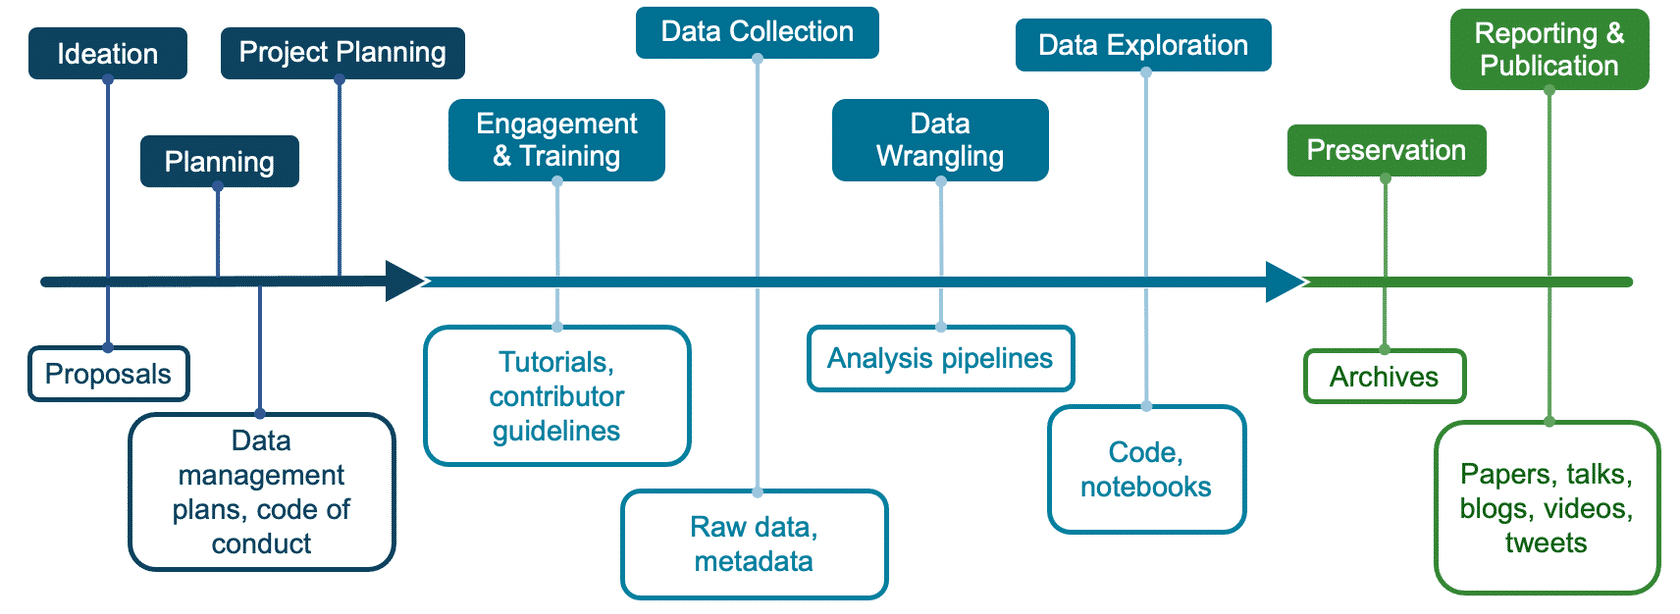
\includegraphics[width=0.9\textwidth]{img/research_cycle.png}
		\label{fig:research_cycle}
		\caption{Source: \href{https://openscience101.org}{OpenScience101.org}}
	\end{figure}
\end{frame}

\begin{frame}
	\frametitle{Use, make, share open results}
	\begin{figure}
		\centering
		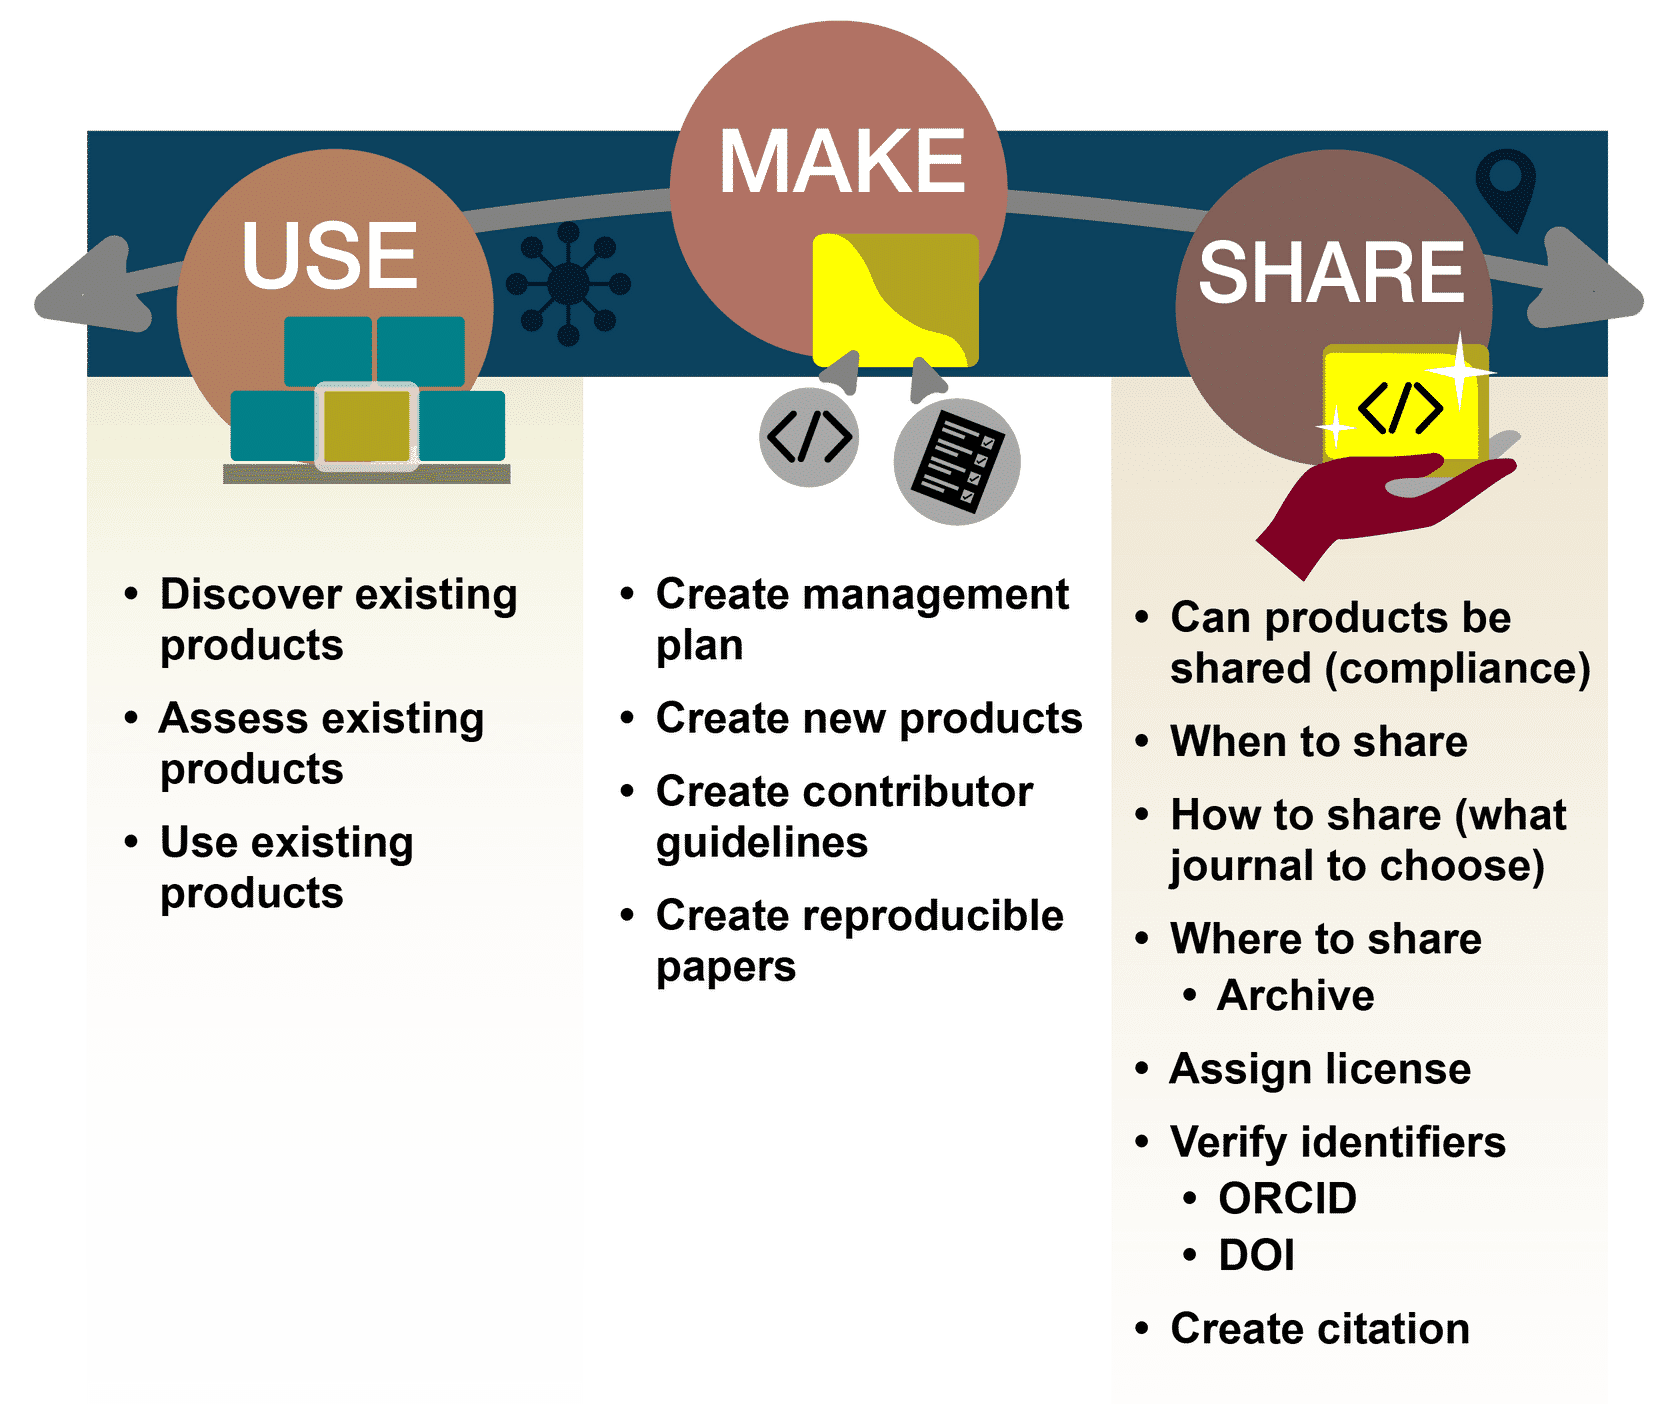
\includegraphics[width=0.5\textwidth]{img/use_make_share.png}
		\label{fig:use_make_share}
		\caption{Source: \href{https://openscience101.org}{OpenScience101.org}}
	\end{figure}
\end{frame}


\subsection{Bibliometrics}


\begin{frame}
	\frametitle{What is bibliometric analysis?}
	\begin{itemize}
		\item Bibliometrics is the measurement of physical units of 
            publications, bibliographic citations, and surrogates for 
            them~\cite{broadus1987}.
		\item The bibliometric methodology encapsules the application of
		      quantitative techniques (i.e., bibliometric analysis --- e.g.,
              citation analysis) on bibliometric data (e.g., units of 
              publication and citation)~\cite{donthu2021}.
	\end{itemize}
\end{frame}

\begin{frame}
	\frametitle{Bibliographic databases}
	\begin{columns}
		\begin{column}{0.5\textwidth}
			\begin{itemize}
				\item \href{https://www.scopus.com}{Scopus}.
				\item \href{https://www.webofknowledge.com}{Web of science}.
			\end{itemize}
		\end{column}
		\begin{column}{0.5\textwidth}
			\begin{figure}
				\centering
				
\includegraphics[width=0.9\textwidth]{logos/scopus.png}\newline
				
\includegraphics[width=0.9\textwidth]{logos/wos.png}
			\end{figure}
		\end{column}
	\end{columns}
\end{frame}

\begin{frame}
    \frametitle{Bibliometrics and LLMs}
    \begin{columns}
		\begin{column}{0.5\textwidth}
            \begin{itemize}
                \item \emph{Large language models reveal big disparities in 
                    current wildfire research}~\cite{lin2024}.
                \item This is a potential new trend in bibliometric analysis.
                \item Feed database data into LLM (ChatGPT).
                \item Extract, besides bibliometric information, localization
                    of AOI.
            \end{itemize}
        \end{column}
		\begin{column}{0.5\textwidth}
            \begin{figure}
                \centering
                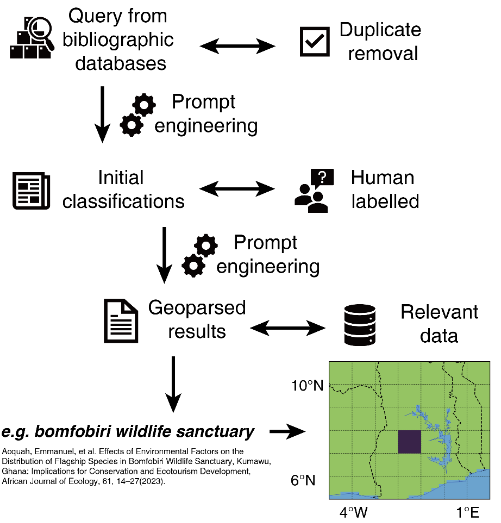
\includegraphics[width=0.8\textwidth]
                {img/lin2024_workflow.png}
                \caption{Source:~\cite{lin2024}.}
            \end{figure}
        \end{column}
    \end{columns}
\end{frame}



\section{Method}



\begin{frame}
    Method.
\end{frame}


\subsection{Definitions}


\begin{frame}
	\frametitle{Documents and references}
	\begin{itemize}
		\item \emph{Document (or citing document)}: Scientific document 
            (article, review, conference proceeding, etc.) included in a 
            bibliographic collection.
		\item \emph{Reference (or cited reference)}: Scientific document 
            included in at least one of the reference lists (bibliography) of 
            the document set. Then \emph{"a reference is cited by one or more 
            documents"}~\cite{aria2017}.
		\item \emph{Cited document}: Scientific document included in a
		      bibliographic collection and, at the same time, it is cited in at 
              least one other document in the collection. Cited documents are a 
              subset of the reference set.
	\end{itemize}
\end{frame}

\begin{frame}
	\frametitle{Global and local citations}
	\begin{columns}
		\begin{column}{0.5\textwidth}
			Global citations.
			\begin{itemize}
				\item Measures the number of citations a document has received 
                    from documents contained in the entire database (e.g. WoS 
                    or Scopus).
				\item Measures the impact of a document in the whole 
                    bibliographic database.
				\item For many documents, a large part of global citations 
                    could come from other disciplines!
			\end{itemize}
		\end{column}
		\begin{column}{0.5\textwidth}
			Local citations.
			\begin{itemize}
				\item Measures the number of citations a document has received 
                    from documents included in the analyzed collection.
				\item Is calculated analyzing the whole reference set.
				\item Measures the impact of a document in the analyzed 
                    collection.
			\end{itemize}
		\end{column}
	\end{columns}
\end{frame}

\subsection{Assumptions}

\begin{frame}
	\frametitle{Assumptions}
	\begin{columns}
		\begin{column}{0.5\textwidth}
        \begin{itemize}
            \item We assumed that TreesLab's publications are a study subject.
        \end{itemize}
        \end{column}
		\begin{column}{0.5\textwidth}
            
\includegraphics[width=0.8\textwidth]{logos/trees-color-h_2.png}
        \end{column}
	\end{columns}
\end{frame}

\begin{frame}
	\frametitle{Method}
	\begin{columns}
		\begin{column}{0.5\textwidth}
			\begin{enumerate}
				\item Get TreesLab publications' DOIs.
				\item Query databases.
                \item Run analysis.
			\end{enumerate}
		\end{column}
		\begin{column}{0.5\textwidth}
			\begin{figure}
				\centering
				
\includegraphics[width=0.2\textwidth]{logos/logo_doi.png}
                
\includegraphics[width=0.4\textwidth]{logos/logo_orcid.png}
                
\includegraphics[width=0.35\textwidth]{logos/zotero.jpg}\newline
				
\includegraphics[width=0.45\textwidth]{logos/scopus.png}
				
\includegraphics[width=0.45\textwidth]{logos/wos.png}\newline
                
\includegraphics[width=0.27\textwidth]{logos/Rlogo.png}
				
\includegraphics[width=0.25\textwidth]{logos/bibliometrix.png}
			\end{figure}
		\end{column}
	\end{columns}
\end{frame}


\subsection{Get TREES Lab publications' DOIs}


\subsubsection{TreesLab publications}

\begin{frame}
	\frametitle{TreesLab publications}
	\begin{columns}
		\begin{column}{0.5\textwidth}
            What constitutes a TreesLab's publication?
			\begin{itemize}
                \item Any publication whose authors agree to add it to the  
                    TreesLab's publication list.
			\end{itemize}
            \vspace{\baselineskip}
            Who are the members of TreesLab?
			\begin{itemize}
                \item Researchers, pos\-docs, Phd \& masters students who 
                    consent on being part of the TreesLab. 
			\end{itemize}
		\end{column}
		\begin{column}{0.5\textwidth}
			\begin{figure}
				\centering
				
\includegraphics[width=0.7\textwidth]{logos/trees-color-h_2.png}
			\end{figure}
		\end{column}
	\end{columns}
\end{frame}

\begin{frame}
	\frametitle{TreesLab publication list}
	\begin{columns}
		\begin{column}{0.5\textwidth}
            \begin{itemize}
                \item The publication list is available using Zotero, both 
                    online (click
                  \href{https://www.zotero.org/groups/5304570/treeslab/library}
                    {here}) and as a desktop application.
                \item Currently, it has 306 items (2024-04-17).
                \item To add a publication, send its DOI to the TreesLab' 
                    mailing list.
                \item Publications wihtout DOI (e.g. GeoInfo, SBSR) should be
                    added to online document \emph{treeslab\_sem\_doi} (click 
\href{https://docs.google.com/document/d/1pnIX_u3Si7J9OBJ1drsbBws5Fgrju_gM4Iyv_DvEw7g/edit?usp=sharing}
                    {here}).
                \item TreesLab's Zotero Group is called \emph{treeslab}.
                \item The former list (Mendeley) is deprecated.
            \end{itemize}
		\end{column}
		\begin{column}{0.5\textwidth}
			\begin{figure}
				\centering
				
\includegraphics[width=0.5\textwidth]{logos/zotero.jpg}
                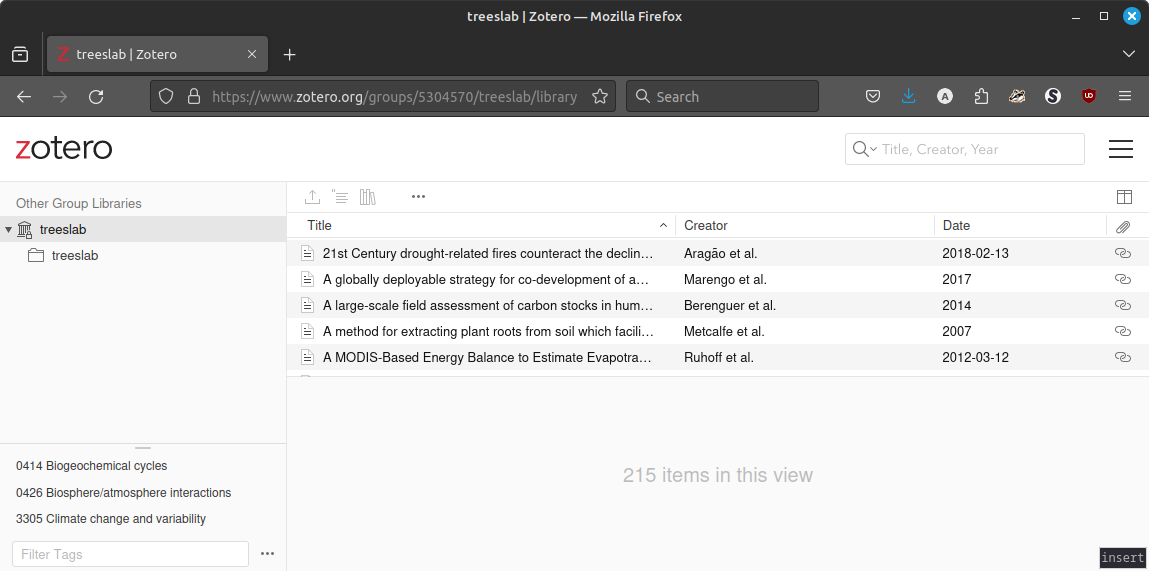
\includegraphics[width=0.9\textwidth]{img/zotero_treeslab.png}
			\end{figure}
		\end{column}
	\end{columns}
\end{frame}

\begin{frame}
    \frametitle{TreesLab Publications' data}
    \begin{columns}
        \begin{column}{0.5\textwidth}
            \begin{itemize}
                \item TreesLab has a Zenodo Community (click 
            \href{https://zenodo.org/communities/treeslab}{here}).
        \item Currently, it has 16 open and 2 restricted datasets 
            (2024-04-017).
                \item To become a member, go to Zenodo, click on communities, 
                    search for \emph{treeslab}, and follow the instructions.
                \item Upload your paper's data (no membership required). 
                \item Make a request to the TreesLab community's administrators 
                    to include your paper's data.
            \end{itemize} 
        \end{column}
        \begin{column}{0.5\textwidth}
            \begin{figure}
                \centering
                
\includegraphics[width=0.4\textwidth]{logos/zenodo.png}
                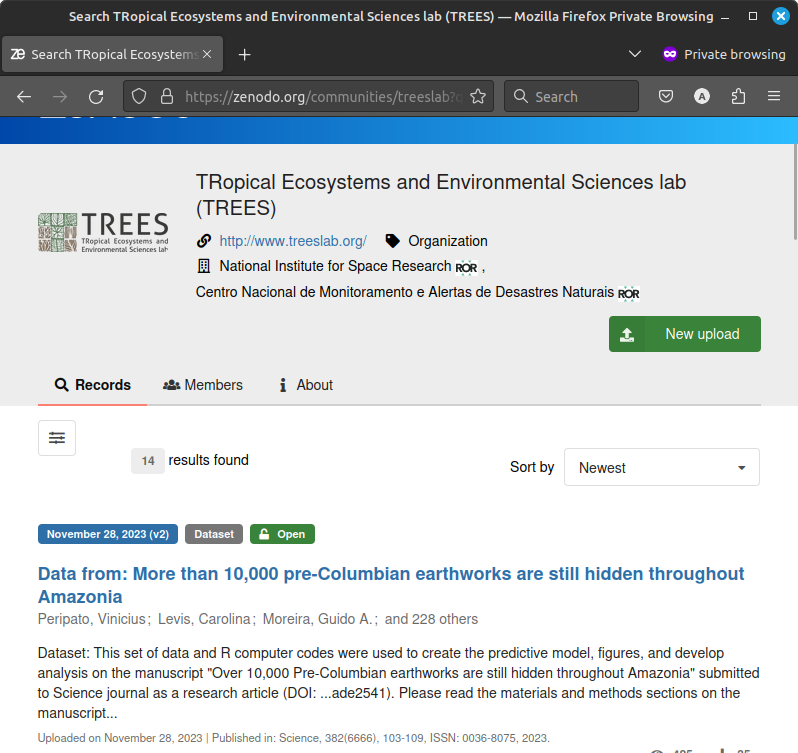
\includegraphics[width=0.8\textwidth]{img/zenodo_treeslab.png}
            \end{figure}
        \end{column}
    \end{columns}
\end{frame}


\subsection{Query Scopus and Web of Science}


\begin{frame}
    \frametitle{From publication list to DOIs}
    \begin{columns}
        \begin{column}{0.5\textwidth}
            \begin{enumerate}
                \item Use Zotero to export publication list to BibTex format.
                \item Use Bash script to extract DOIs to a text file.
                \item Use a text editor to build queries for both Scopus and 
                    Web Of Science databases.
            \end{enumerate}
        \end{column}
        \begin{column}{0.5\textwidth}
			\begin{figure}
				\centering
				
\includegraphics[width=0.5\textwidth]{logos/zotero.jpg}
                
\includegraphics[width=0.5\textwidth]{logos/bash.png}
                
\includegraphics[width=0.6\textwidth]{logos/neovim-logo.png}
			\end{figure}
        \end{column}
    \end{columns}
\end{frame}

\begin{frame}
	\frametitle{Scopus and Web of Science at INPE}
	\begin{columns}
		\begin{column}{0.5\textwidth}
			\begin{itemize}
				\item To run the queries, use a computer at INPE and your Café 
                    login.
                \item The database interface offers advanced options, where you
                    can type complex queries.
                \item Store the resutla as either CSV or Plain Text for 
                    further processing.
			\end{itemize}
		\end{column}
		\begin{column}{0.5\textwidth}
			\begin{figure}
				\centering
				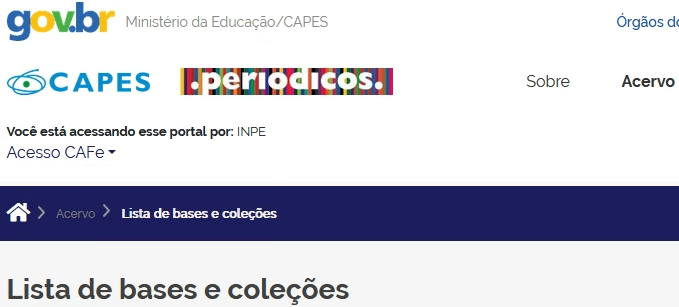
\includegraphics[width=0.9\textwidth]{img/inpe_cafe.png}
			\end{figure}
		\end{column}
	\end{columns}
\end{frame}

\subsection{Run analysis using \textit{R}}

\begin{frame}
	\frametitle{Bibliometrix}
	\begin{columns}
		\begin{column}{0.5\textwidth}
			\begin{itemize}
				\item R package for bibliometric analysis~\cite{aria2017}.
				\item It allows quantitative research in bibliometrics and
				      scientometrics.
				\item Statistical analysis of publications.
				\item Useful for performance evaluation and policymaking.
				\item It includes a Web Application (biblioshiny) for 
                    non-programmers!
			\end{itemize}
		\end{column}
		\begin{column}{0.5\textwidth}
			\begin{figure}
				\centering
				
\includegraphics[width=0.8\textwidth]{logos/bibliometrix.png}
			\end{figure}
		\end{column}
	\end{columns}
\end{frame}

\begin{frame}
    \frametitle{Bibliometrix field tags}
    \begin{columns}
		\begin{column}{0.5\textwidth}
            \begin{itemize}
                \item Some of the column names used by Bibliometrix.
                \item Find the complete list clicking 
     \href{https://www.bibliometrix.org/documents/Field_Tags_bibliometrix.pdf}
                    {here}.
            \end{itemize}
		\end{column}
		\begin{column}{0.5\textwidth}
            \begin{figure}
                \centering
                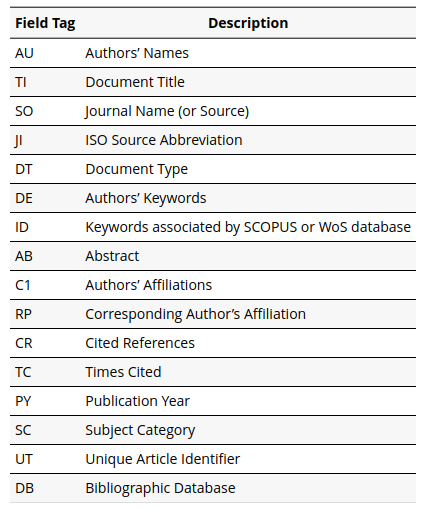
\includegraphics[width=0.7\textwidth]
                {img/bibliometrix_field_tags.png}
                \caption{Source: 
\href{https://www.bibliometrix.org/vignettes/Data-Importing-and-Converting.html}
                {Bibliometrix - Data Importing and Converting}.}
            \end{figure}
		\end{column}
    \end{columns}
\end{frame}



\section{Results} 



\begin{frame}
    Results.
\end{frame}


\subsection{Results overview}


\begin{frame}
	\frametitle{Overview}
	\centering
	\small
	
\begin{tabular}{ll}
\toprule
Description & Results\\
\midrule
Timespan & 2003:2024\\
Sources (Journals, Books, etc) & 84\\
Documents & 218\\
Annual Growth Rate \% & 10.41\\
Document Average Age & 7.43\\
\addlinespace
Average citations per doc & 82.65\\
References & 1\\
Author's Keywords (DE) & 571\\
Authors & 1371\\
Authors of single-authored docs & 1\\
\addlinespace
Co-Authors per Doc & 15.6\\
International co-authorships \% & 86.24\\
\bottomrule
\end{tabular}
\end{frame}

\begin{frame}
	\frametitle{Documents by type}
	\centering
	\small
	
\begin{tabular}{lr}
\toprule
Description & Results\\
\midrule
article & 181\\
letter & 12\\
review & 9\\
editorial material & 6\\
article; proceedings paper & 2\\
\addlinespace
biographical-item & 1\\
correction & 1\\
\bottomrule
\end{tabular}
\end{frame}

\begin{frame}
	\begin{columns}
		\begin{column}{0.5\textwidth}
			\frametitle{Authors' productivity}
			\centering
			\small
			
\begin{tabular}{lr}
\toprule
Authors & Articles\\
\midrule
ARAGAO L & 144\\
ANDERSON L & 98\\
MALHI Y & 59\\
SHIMABUKURO Y & 42\\
PHILLIPS O & 31\\
\addlinespace
MATAVELI G & 24\\
SILVA C & 24\\
ARAI E & 21\\
BAKER T & 20\\
DALAGNOL R & 20\\
\bottomrule
\end{tabular}
		\end{column}
		\begin{column}{0.5\textwidth}
			\centering
			\small
			
\begin{tabular}{lr}
\toprule
Authors & Articles Fractionalized\\
\midrule
ARAGÃO L & 13.91\\
ANDERSON L & 13.21\\
SHIMABUKURO Y & 6.04\\
MALHI Y & 5.21\\
ARAI E & 2.43\\
\addlinespace
MATAVELI G & 2.32\\
DE O G & 2.07\\
WAGNER F & 1.94\\
DALAGNOL R & 1.90\\
ARAGAO L & 1.64\\
\bottomrule
\end{tabular}
		\end{column}
	\end{columns}
\end{frame}

\begin{frame}
	\frametitle{Most cited papers}
	\centering
	\small
	
\begin{tabular}{lrrr}
\toprule
Paper & TC & TCperYear & NTC\\
\midrule
NEMANI R, 2003, SCIENCE & 2741 & 124.6 & 1.00\\
BRIENEN R, 2015, NATURE & 783 & 78.3 & 4.31\\
LUYSSAERT S, 2007, GLOBAL CHANGE BIOL & 776 & 43.1 & 3.06\\
MORTON D, 2006, P NATL ACAD SCI USA & 681 & 35.8 & 4.09\\
BARLOW J, 2016, NATURE & 673 & 74.8 & 7.45\\
\addlinespace
MALHI Y, 2009, P NATL ACAD SCI USA & 604 & 37.8 & 4.05\\
ARAGAO L, 2018, NAT COMMUN & 496 & 70.9 & 4.80\\
PHILLIPS O, 2010, NEW PHYTOL & 446 & 29.7 & 3.01\\
GATTI L, 2021, NATURE & 435 & 108.8 & 9.06\\
GATTI L, 2014, NATURE & 373 & 33.9 & 3.43\\
\bottomrule
\end{tabular}
\end{frame}

\begin{frame}
	\frametitle{Most relevant sources}
	\centering
	\scriptsize
	
\begin{tabular}{lr}
\toprule
Sources & Articles\\
\midrule
GLOBAL CHANGE BIOLOGY & 17\\
REMOTE SENSING & 10\\
NEW PHYTOLOGIST & 9\\
SCIENCE & 9\\
BIOGEOSCIENCES & 8\\
\addlinespace
PLANT ECOLOGY AND DIVERSITY & 8\\
NATURE & 7\\
PLOS ONE & 6\\
SCIENTIFIC REPORTS & 6\\
ENVIRONMENTAL RESEARCH LETTERS & 5\\
\addlinespace
FIRE & 5\\
PHILOSOPHICAL TRANSACTIONS OF THE ROYAL SOCIETY B: BIOLOG... & 5\\
\bottomrule
\end{tabular}
\end{frame}

\begin{frame}
	\frametitle{Production over time - sources}
	\begin{figure}
		\centering
		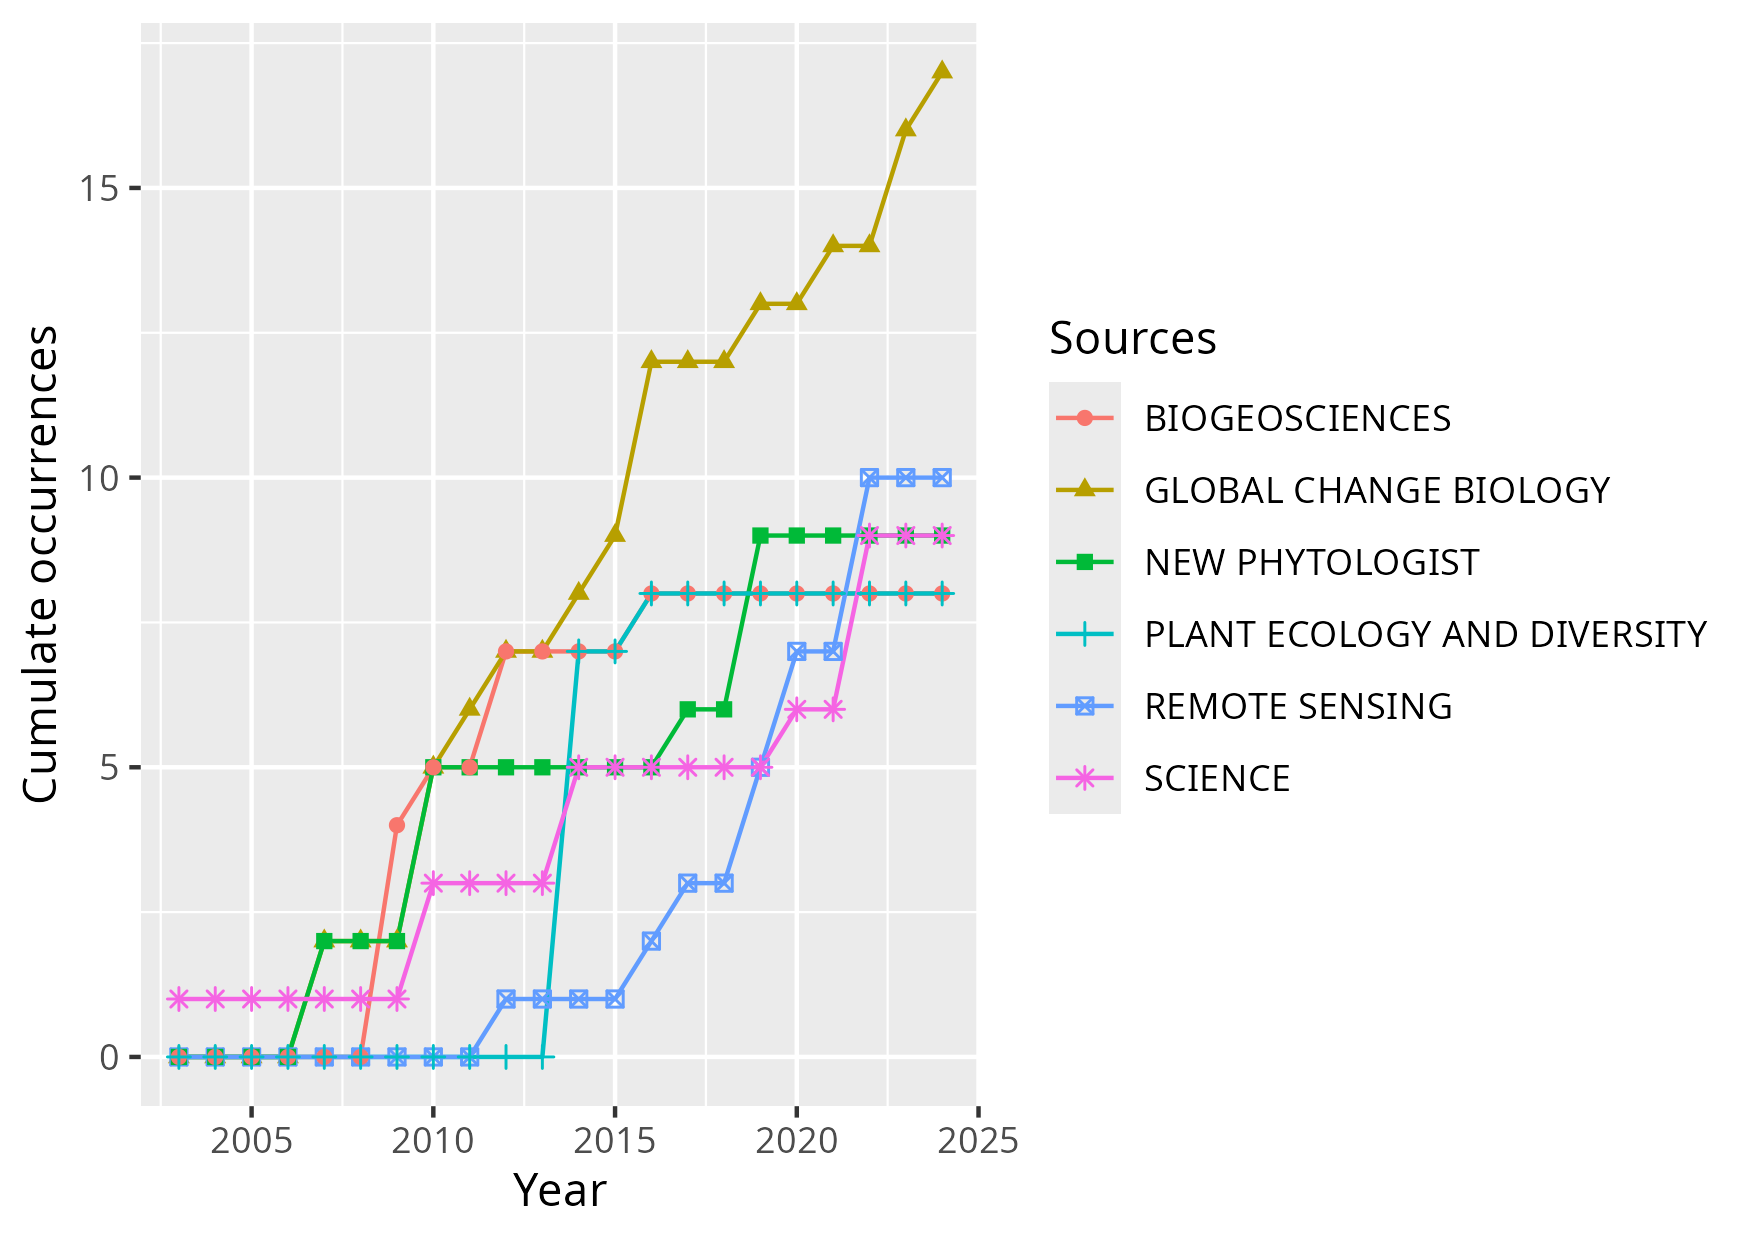
\includegraphics[width=0.8\textwidth]
        {figures/sources_production_over_time.png}
	\end{figure}
\end{frame}

\begin{frame}
	\frametitle{Most relevant keywords}
	\begin{columns}
		\begin{column}{0.5\textwidth}
			\centering
			\scriptsize
			
\begin{tabular}{lr}
\toprule
Author Keywords (DE) & Articles\\
\midrule
AMAZON & 29\\
REMOTE SENSING & 21\\
DEFORESTATION & 19\\
DROUGHT & 17\\
FIRE & 13\\
\addlinespace
TROPICAL FOREST & 13\\
MODIS & 12\\
CLIMATE CHANGE & 11\\
PHENOLOGY & 11\\
TROPICAL FORESTS & 11\\
\bottomrule
\end{tabular}
		\end{column}
		\begin{column}{0.5\textwidth}
			\centering
			\scriptsize
			
\begin{tabular}{lr}
\toprule
Keywords-Plus (ID) & Articles\\
\midrule
DEFORESTATION & 52\\
CLIMATE-CHANGE & 36\\
CARBON & 26\\
RAIN-FOREST & 26\\
TROPICAL FORESTS & 25\\
\addlinespace
FOREST & 23\\
BIOMASS & 20\\
LAND-USE & 20\\
PATTERNS & 20\\
DYNAMICS & 19\\
\bottomrule
\end{tabular}
		\end{column}
	\end{columns}
\end{frame}

\begin{frame}
	\frametitle{Most Productive Authors}
	\begin{figure}
		\centering
		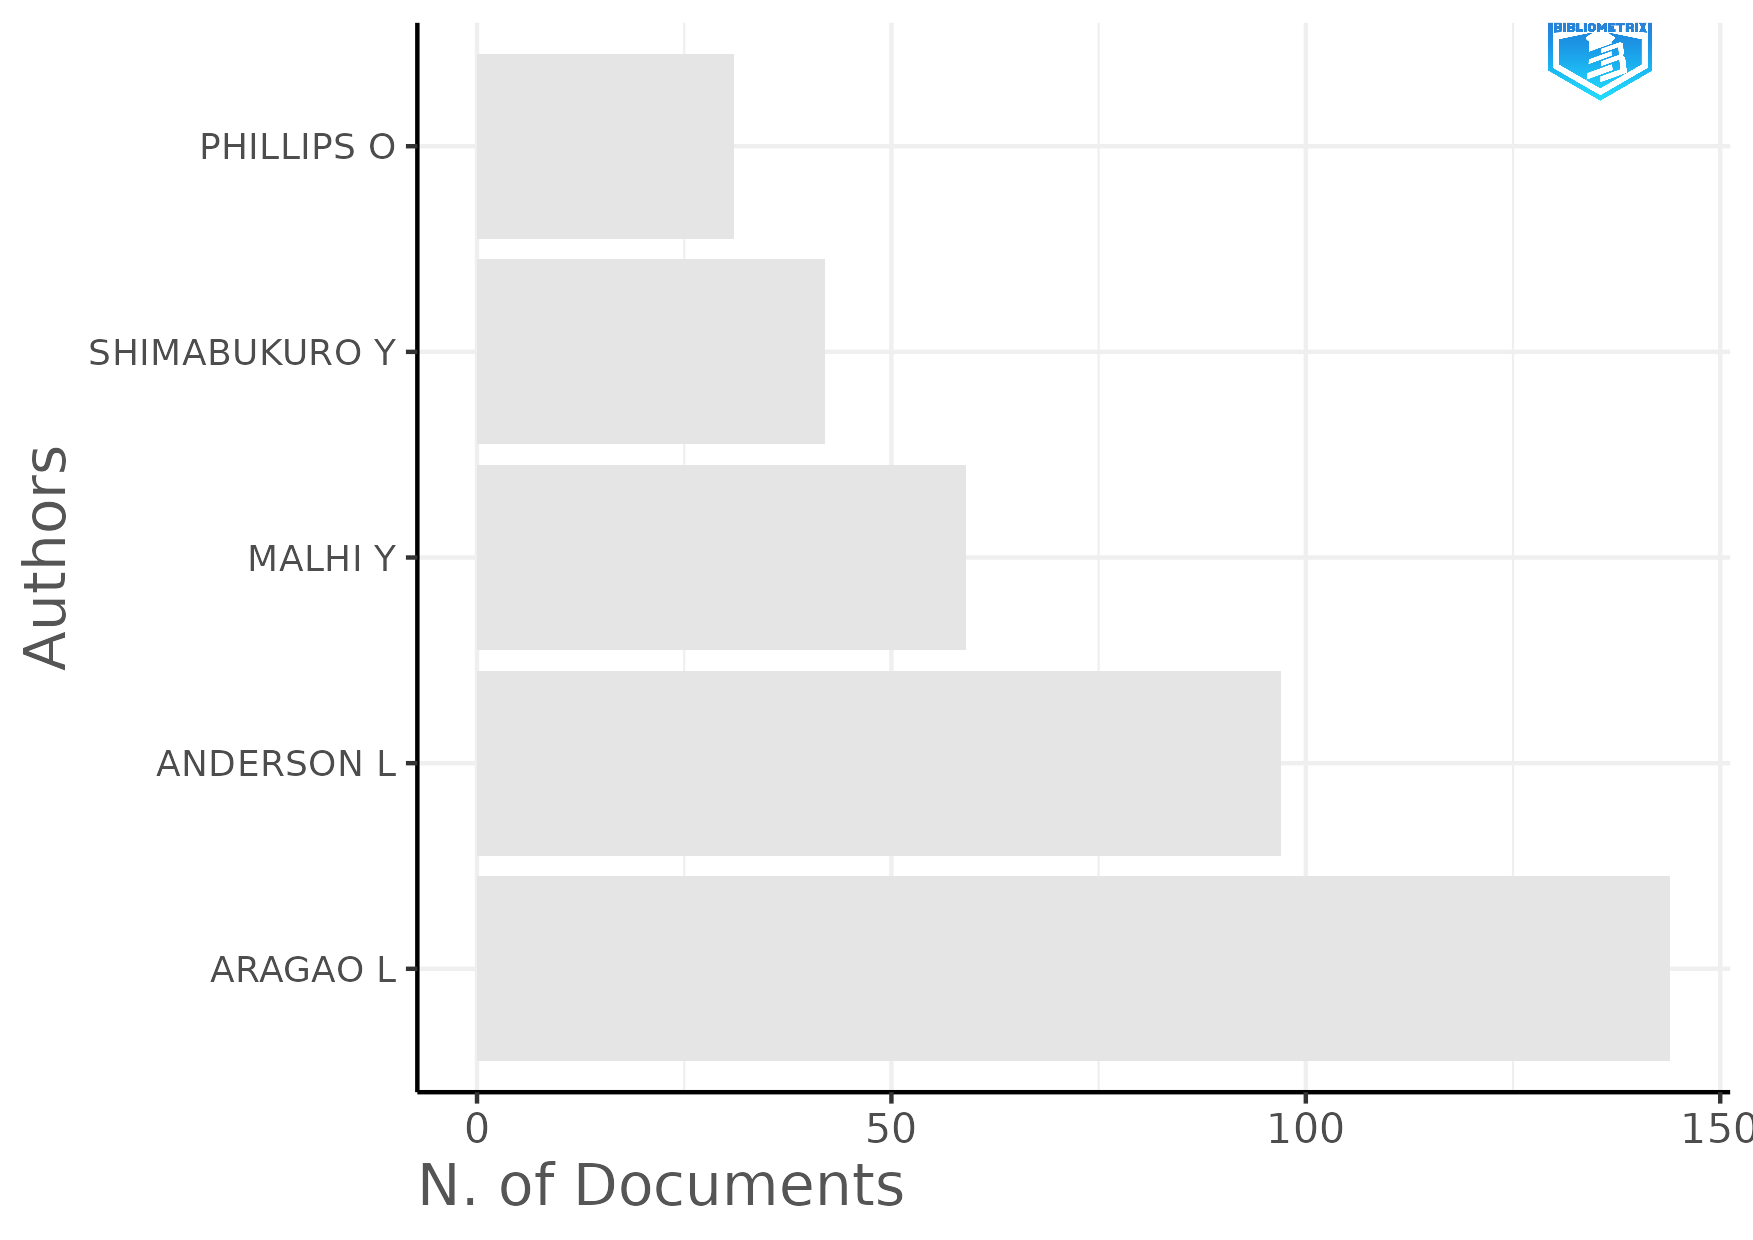
\includegraphics[width=0.7\textwidth]{figures/MostProdAuthors.png}
	\end{figure}
\end{frame}

\begin{frame}
	\frametitle{Most Productive Countries}
	\begin{figure}
		\centering
		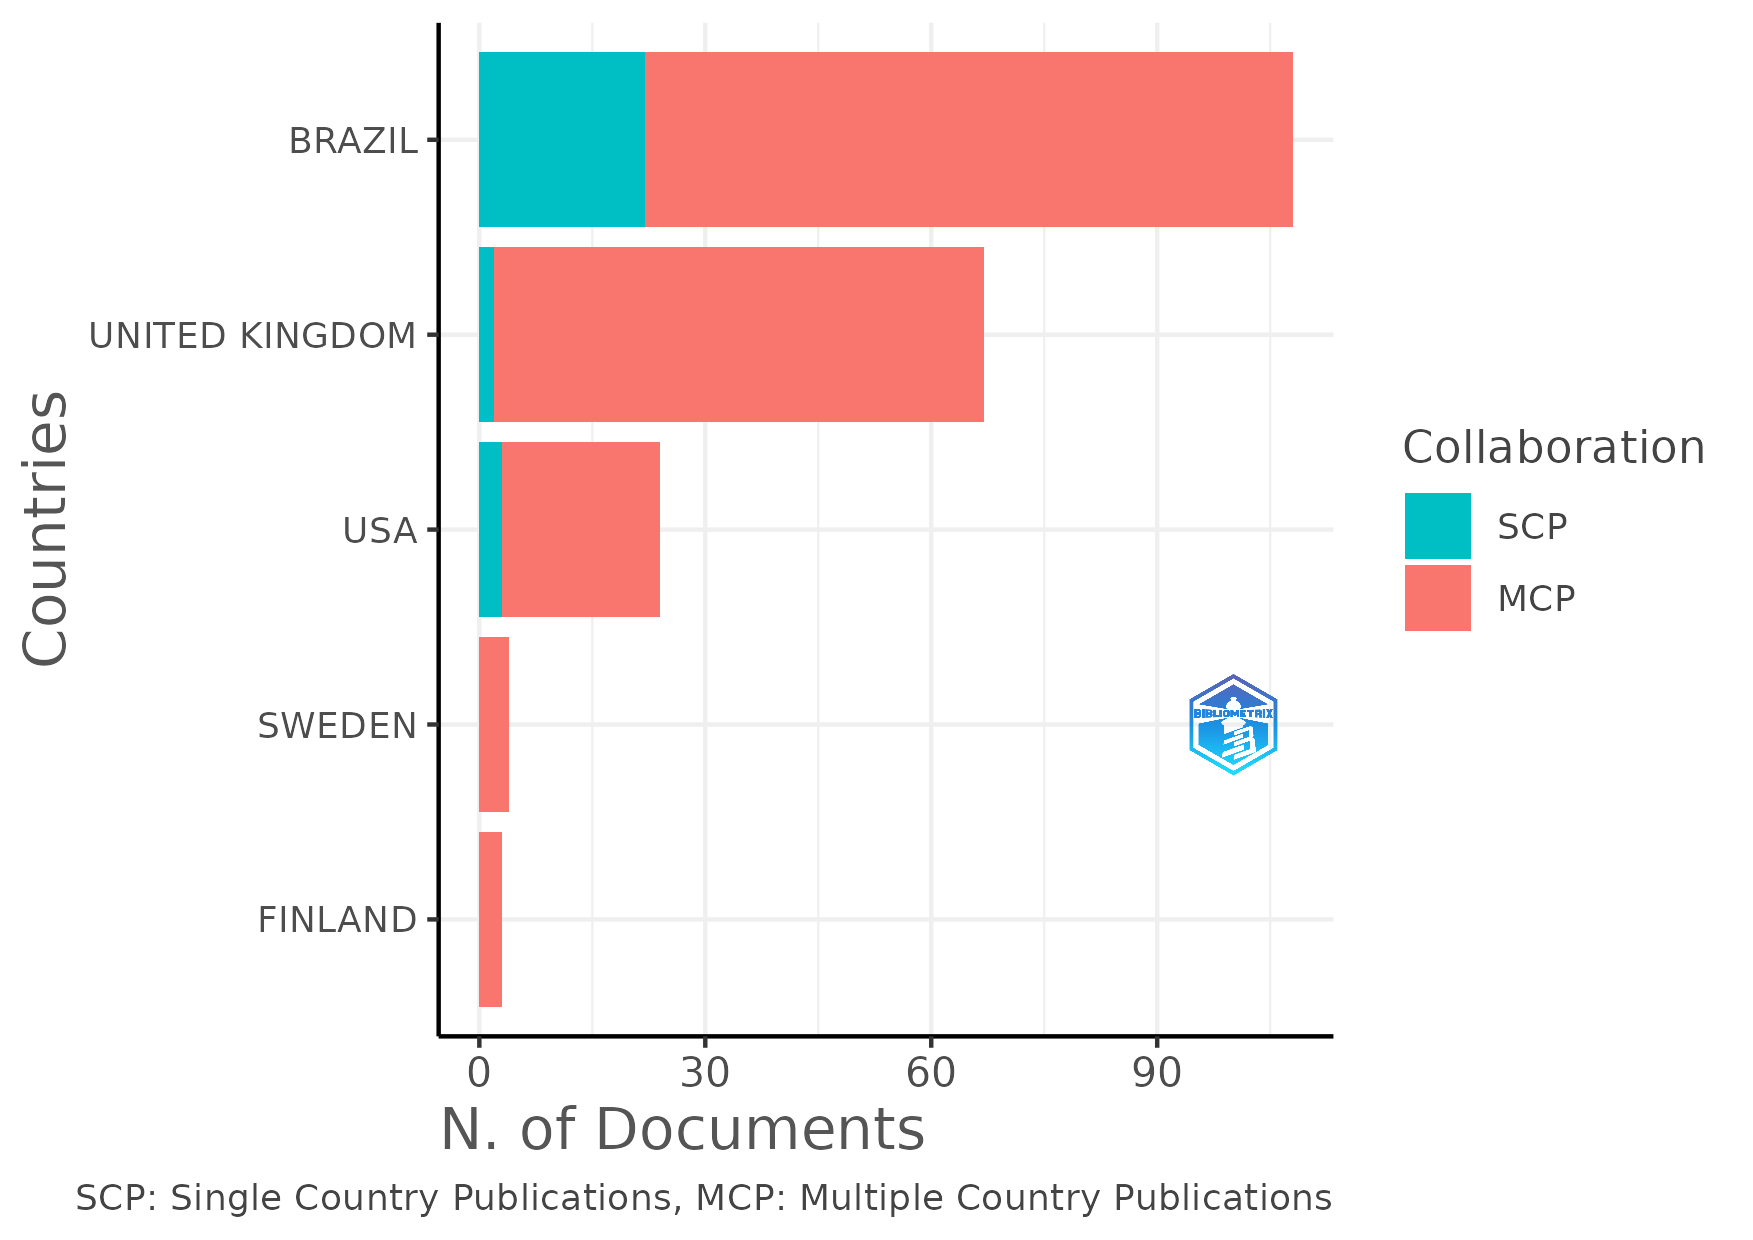
\includegraphics[width=0.7\textwidth]{figures/MostProdCountries.png}
	\end{figure}
\end{frame}

\begin{frame}
	\frametitle{Annual Scientific Production}
	\begin{figure}
		\centering
		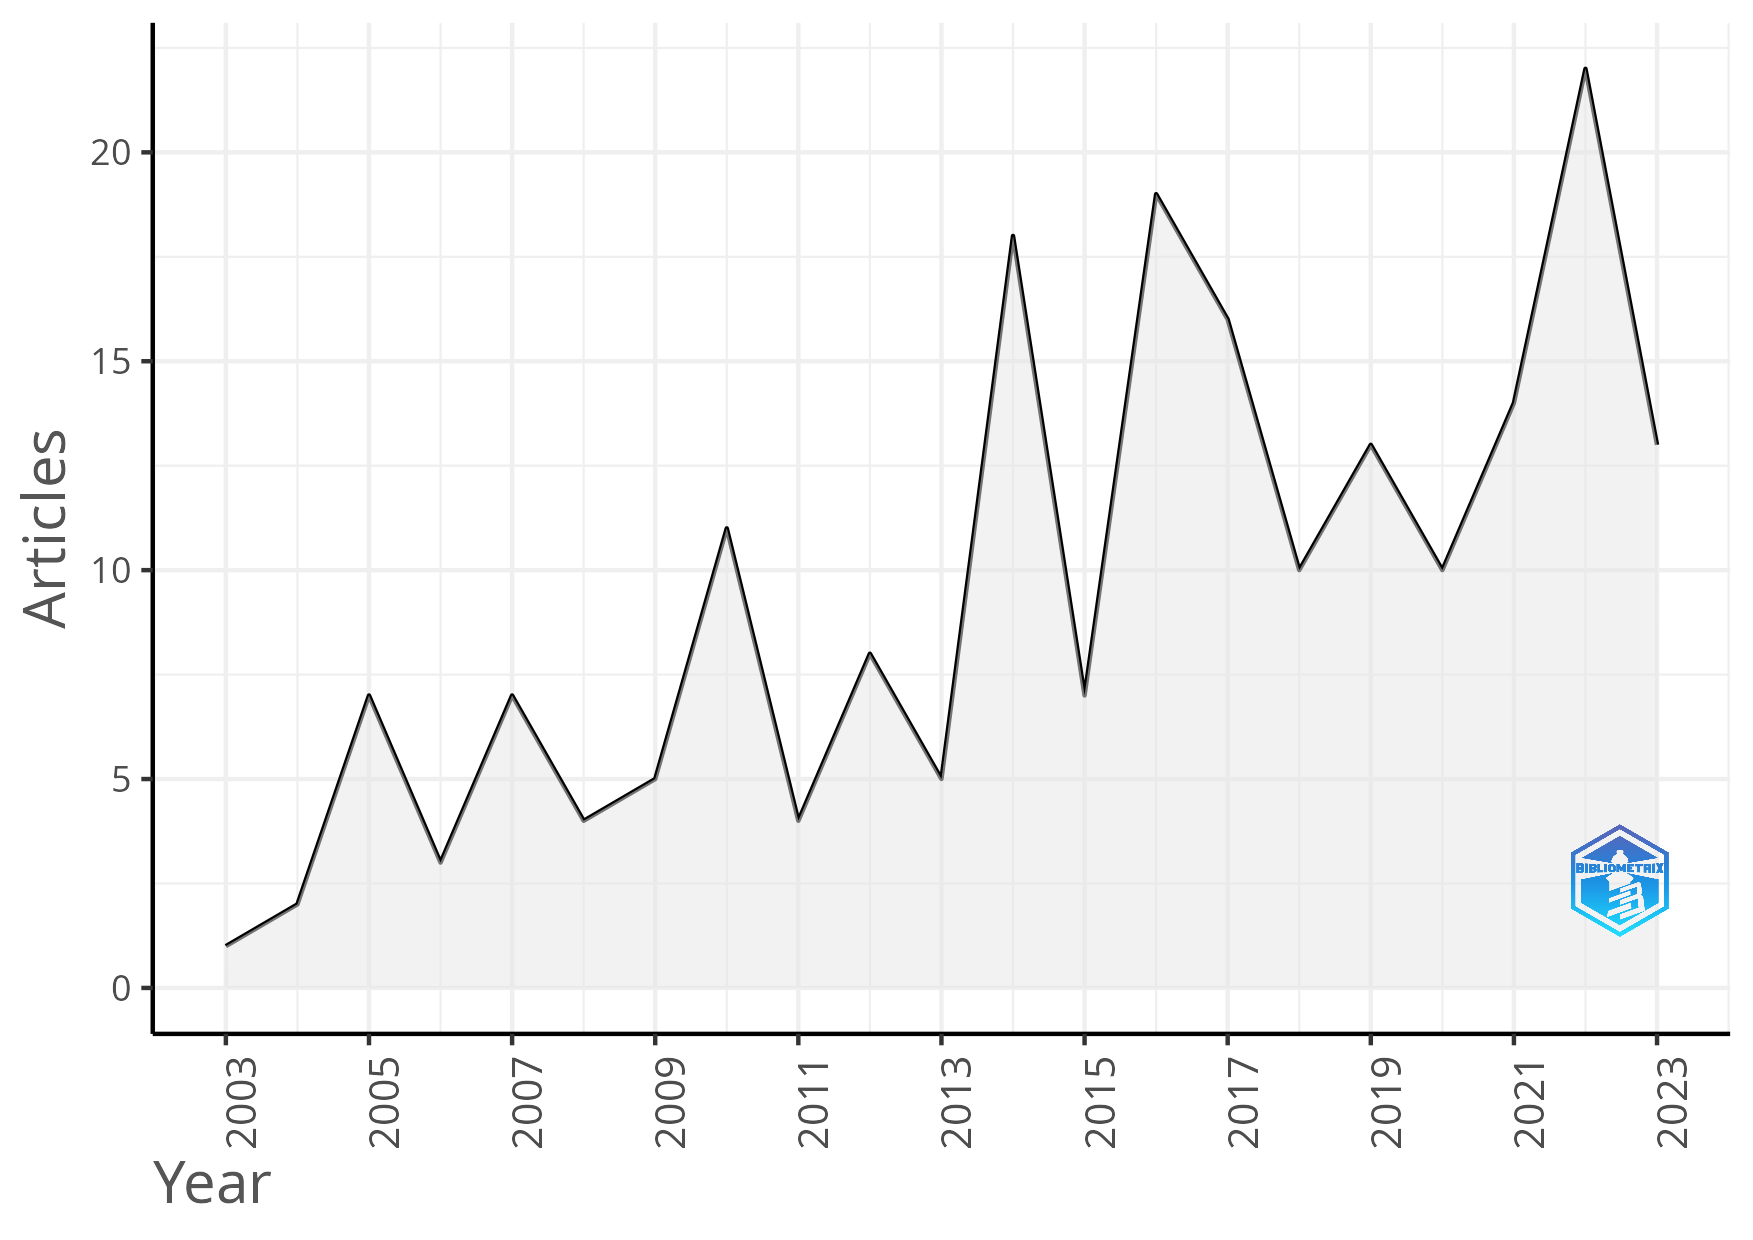
\includegraphics[width=0.7\textwidth]{figures/AnnualScientProd.png}
	\end{figure}
\end{frame}

\begin{frame}
	\frametitle{Average Article Citation per Year}
	\begin{figure}
		\centering
		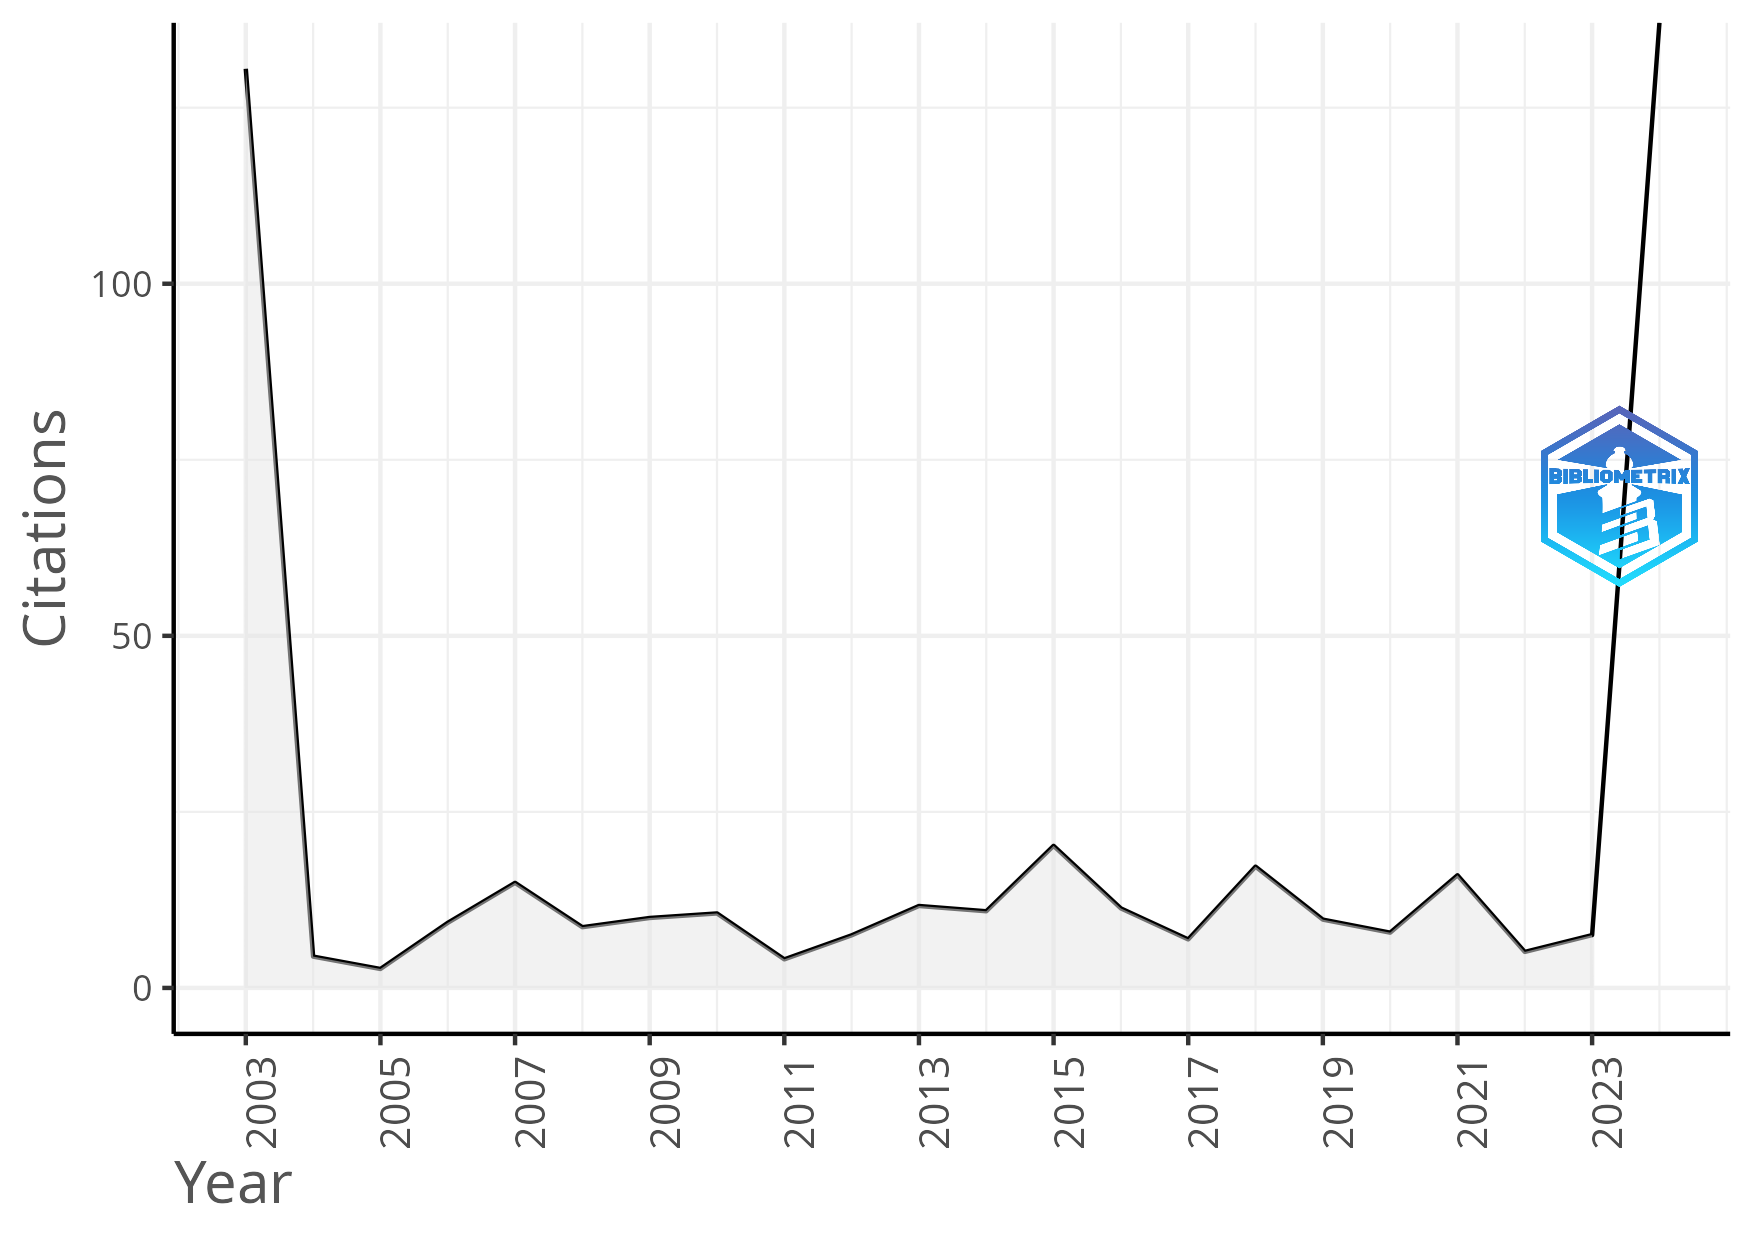
\includegraphics[width=0.7\textwidth]{figures/AverArtCitperYear.png}
	\end{figure}
\end{frame}

\begin{frame}
	\frametitle{Average Total Citation per Year}
	\begin{figure}
		\centering
		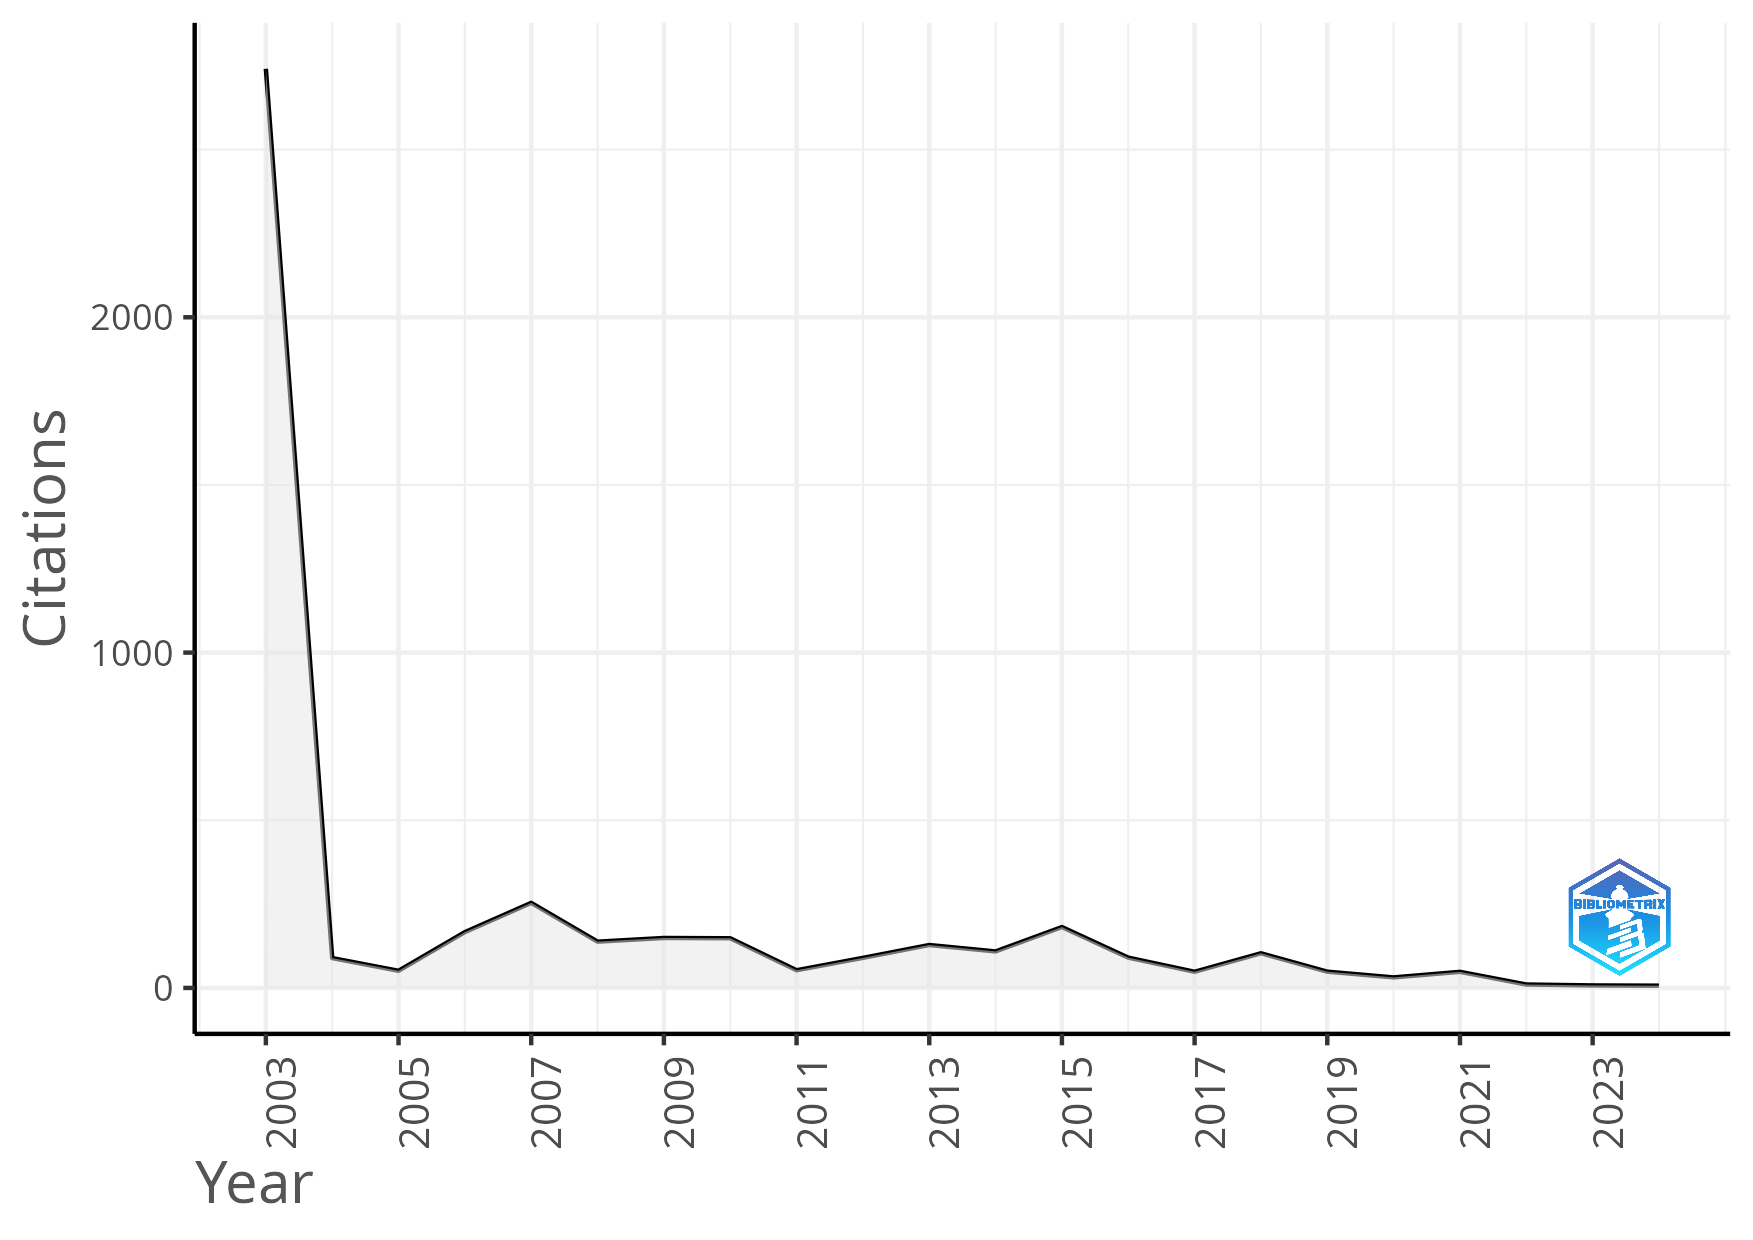
\includegraphics[width=0.7\textwidth]{figures/AverTotCitperYear.png}
	\end{figure}
\end{frame}


\subsection{Knowledge synthesis}


\begin{frame}
	\frametitle{Structures of knowledge}
	\begin{itemize}
		\item Science mapping aims at displaying the structural and dynamic aspects of
		      scientific research~\cite{borner2003}.
		\item \emph{Science mapping} allows investigating scientific knowledge from a
		      statistical point of view:
		      \begin{itemize}
			      \item \emph{Conceptual}: What science talks about; themes and 
                      trends.
			      \item \emph{Intellectual}: How the work of an author 
                      influences a given scientific community.
			      \item \emph{Social}: How authors, institutions, and countries 
                      interact with each other.
		      \end{itemize}
	\end{itemize}
\end{frame}


\subsection{Conceptual structure}


\begin{frame}
	\frametitle{Conceptual structure}
	Represent relations among concepts or words in a set of publications.
    \begin{itemize}
        \item Words whih appear together in a document would be related in a 
            network (co-words network). 
        \item Factorial analysis helps to identify subfields by means of data
            reduction techniques.
        \item Mixed approach.
    \end{itemize}
\end{frame}


\subsection{Thematic map}


\begin{frame}
	\frametitle{The strategic diagram}
	\begin{columns}
		\begin{column}{0.5\textwidth}
			\begin{itemize}
				\item Upper-right: Themes are related externally to concepts applicable
				      to other themes that are conceptually closely related.
				\item Upper-left: Well-developed internal ties but unimportant external
				      ties; marginal importance for the field.
				\item Lower-left: Mainly represents emerging or disappearing themes.
				\item Lower-right: Important for a research field but are not
				      developed.
			\end{itemize}
		\end{column}
		\begin{column}{0.5\textwidth}
			\begin{figure}
				\centering
				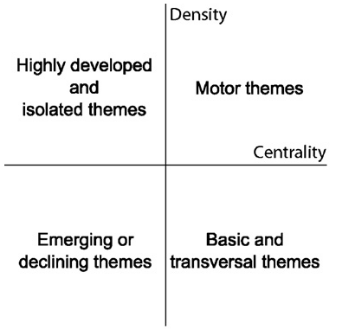
\includegraphics[width=0.8\textwidth]
				{./img/strategic_diagram_cobo2011.png}
				\label{fig:strategic_diagram}
				\caption{The strategic diagram. Source~\cite{cobo2011}}
			\end{figure}
		\end{column}
	\end{columns}
\end{frame}

\begin{frame}
	\frametitle{Thematic map (keyword plus)}
	\begin{figure}
		\centering
		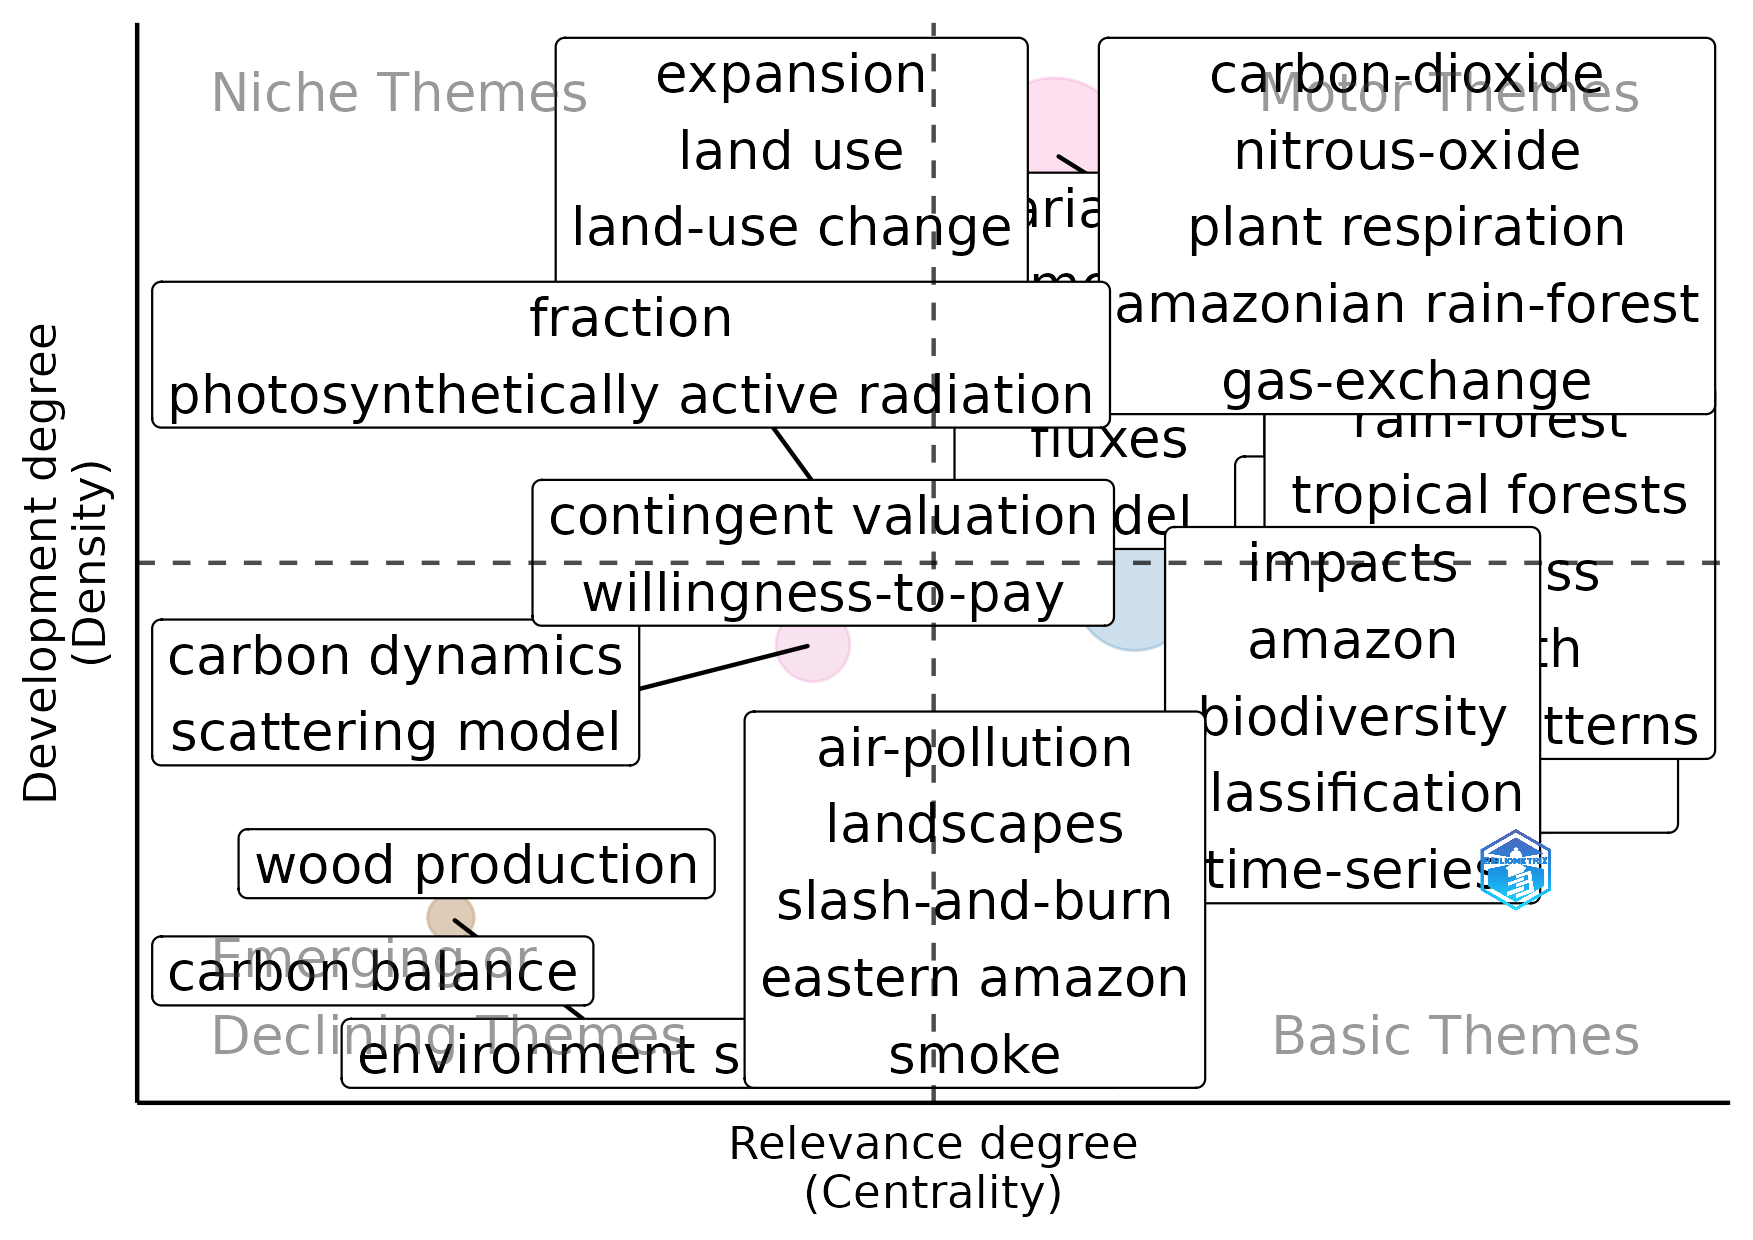
\includegraphics[width=0.7\textwidth]{figures/thematic_map_keyword_plus.png}
	\end{figure}
\end{frame}

\begin{frame}
	\frametitle{Thematic map (authors' keywords)}
	\begin{figure}
		\centering
		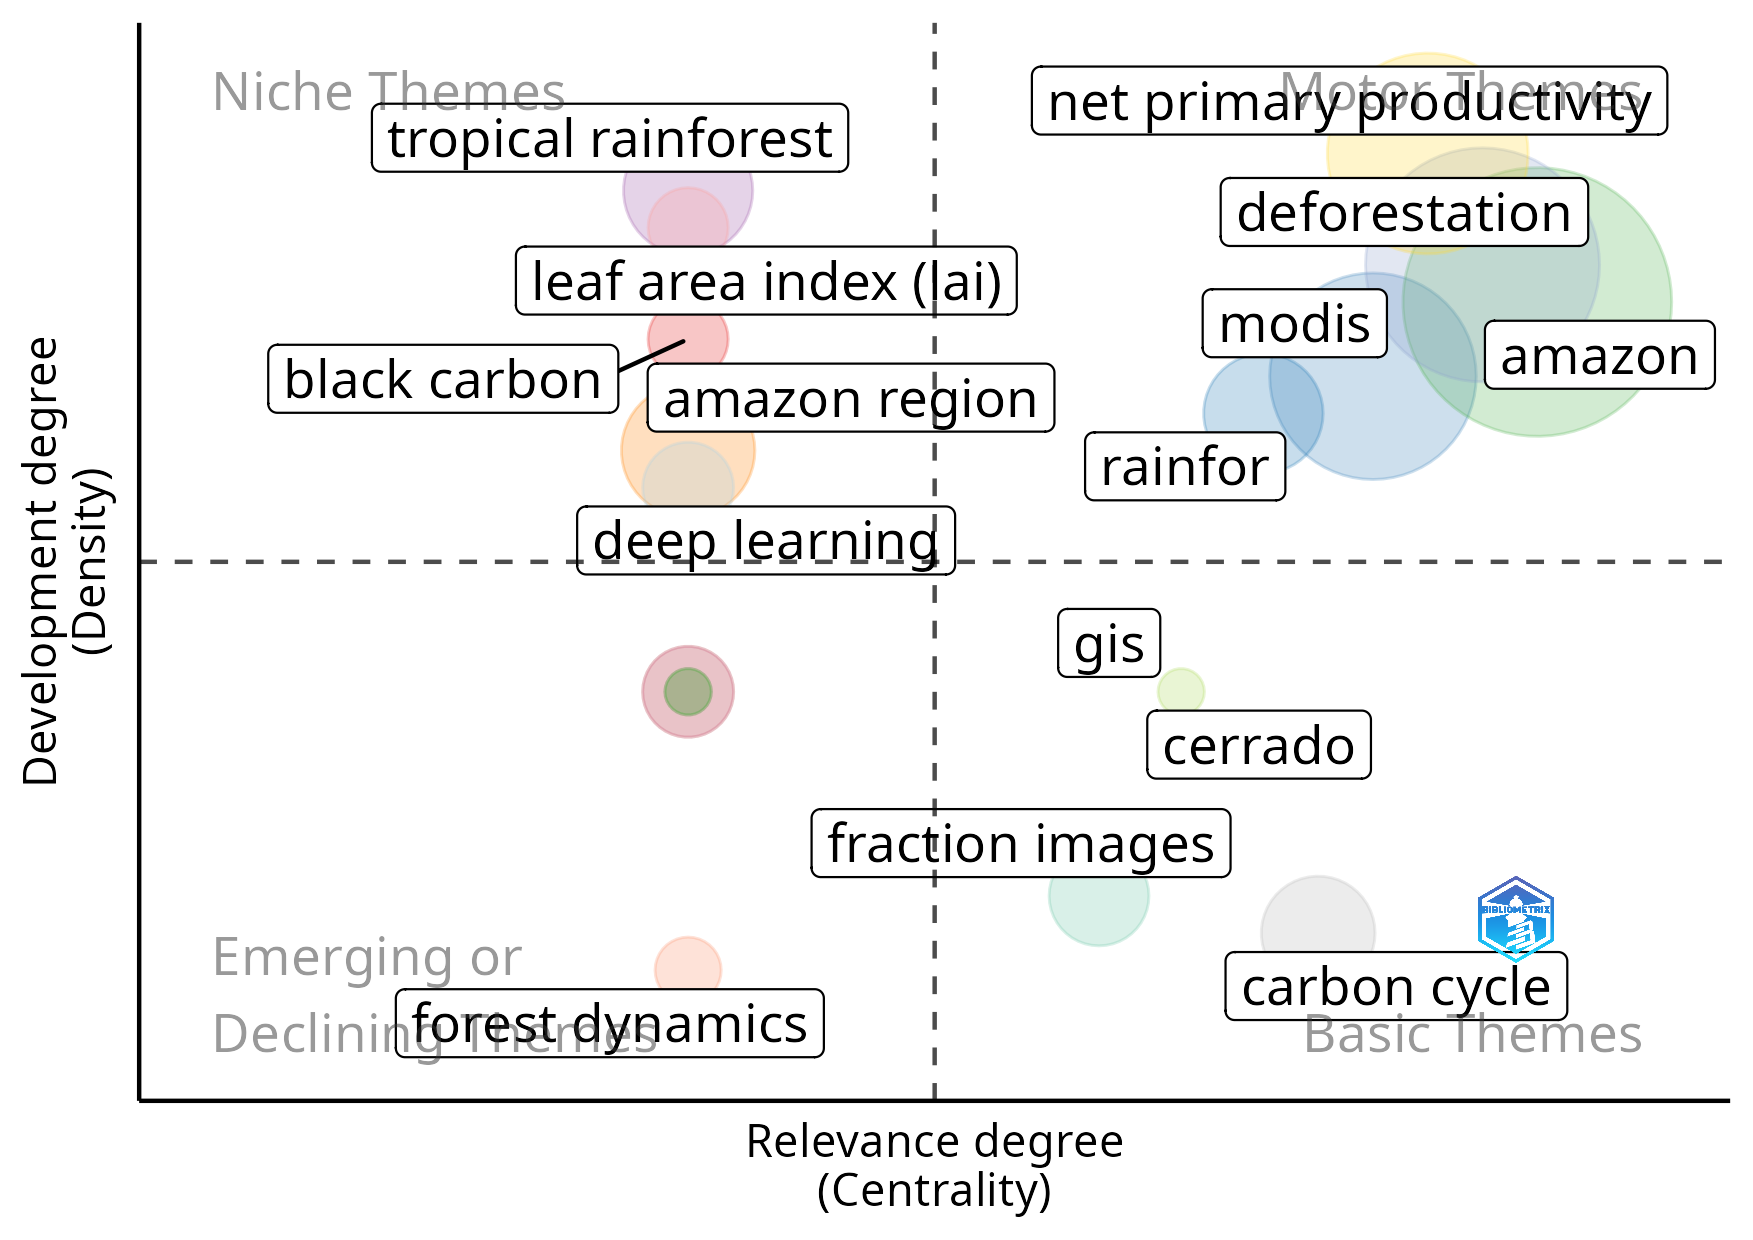
\includegraphics[width=0.7\textwidth]{figures/thematic_map_keyword_authors.png}
	\end{figure}
\end{frame}

\begin{frame}
	\frametitle{Thematic map (titles)}
	\begin{figure}
		\centering
		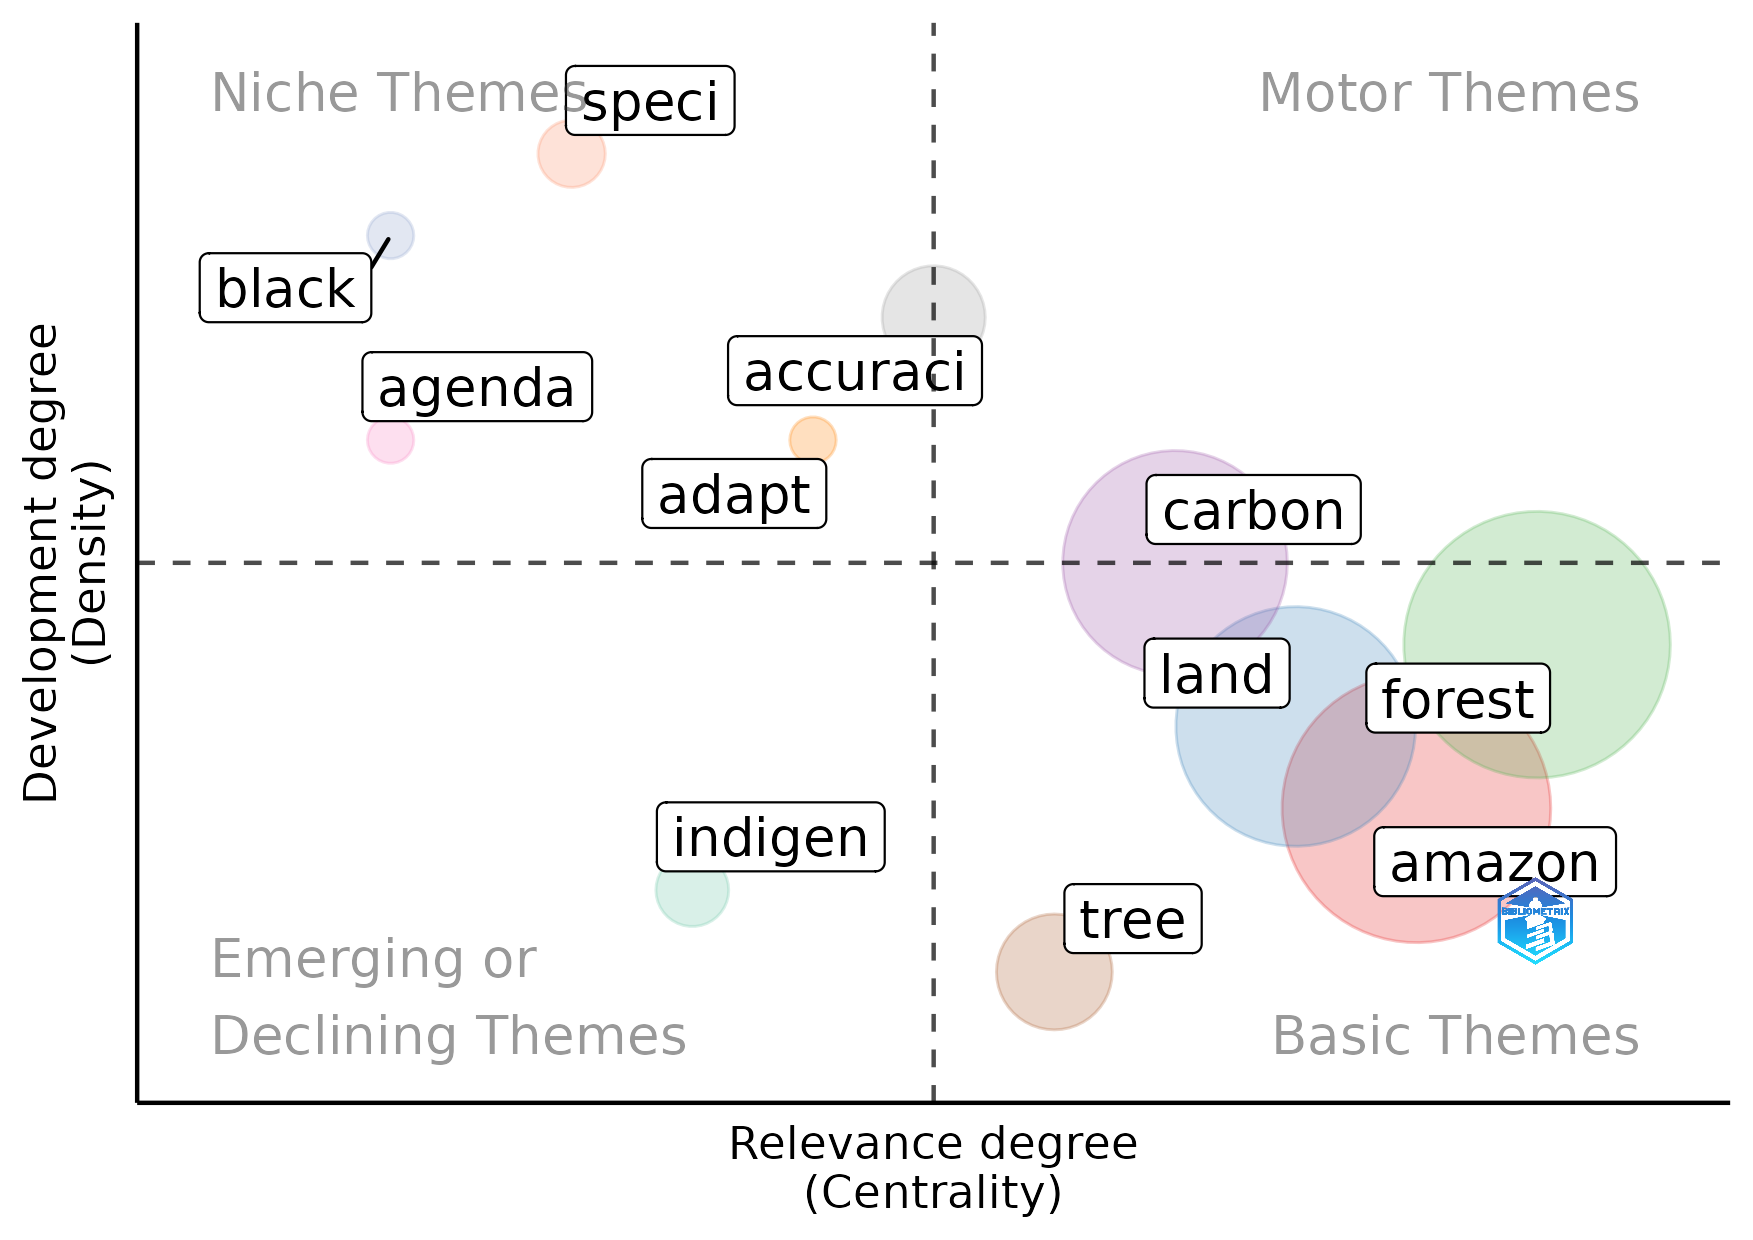
\includegraphics[width=0.7\textwidth]{figures/thematic_map_titles.png}
	\end{figure}
\end{frame}

\begin{frame}
	\frametitle{Thematic map (abstracts)}
	\begin{figure}
		\centering
		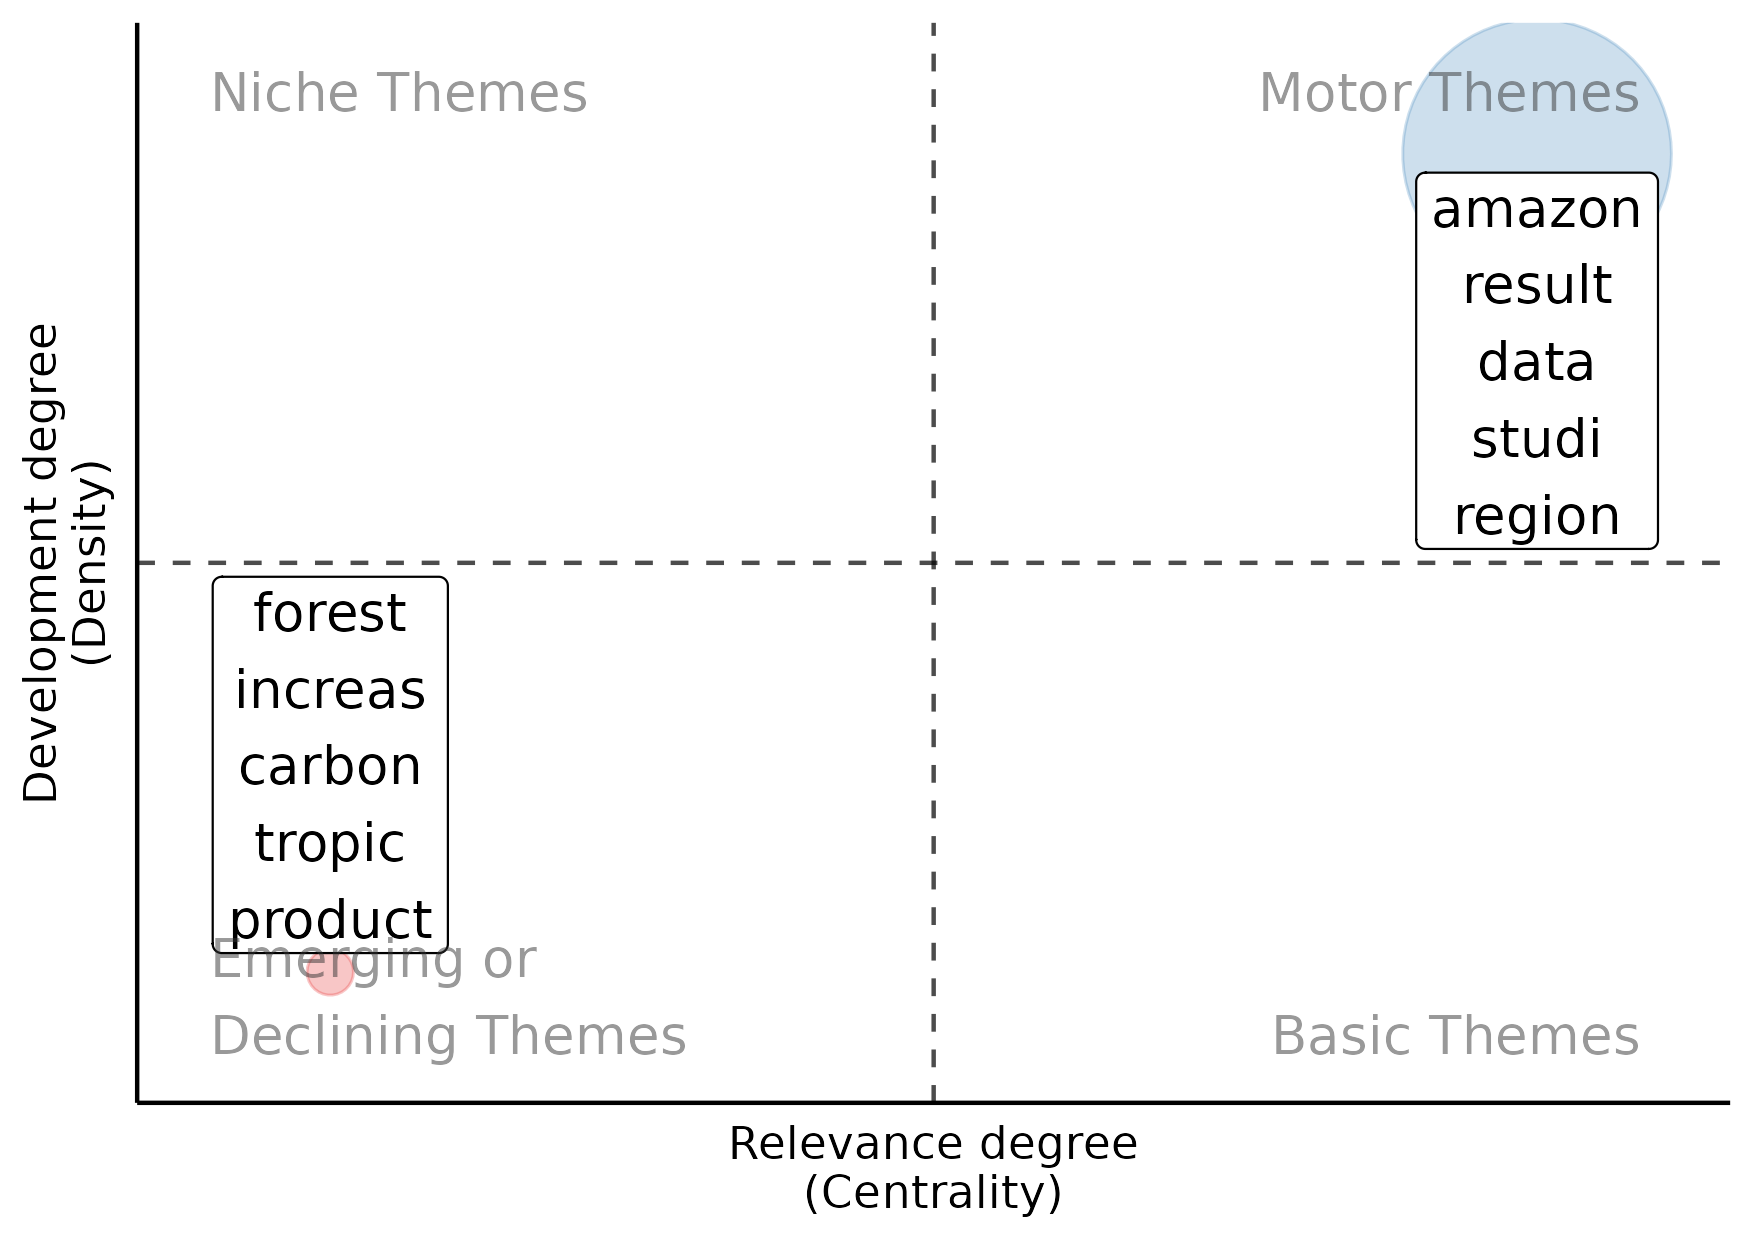
\includegraphics[width=0.7\textwidth]
        {figures/thematic_map_abstracts.png}
	\end{figure}
\end{frame}


\subsection{Thematic evolution}


\begin{frame}
	\frametitle{Thematic evolution - 2003:2007}
    \begin{figure}
        \centering
        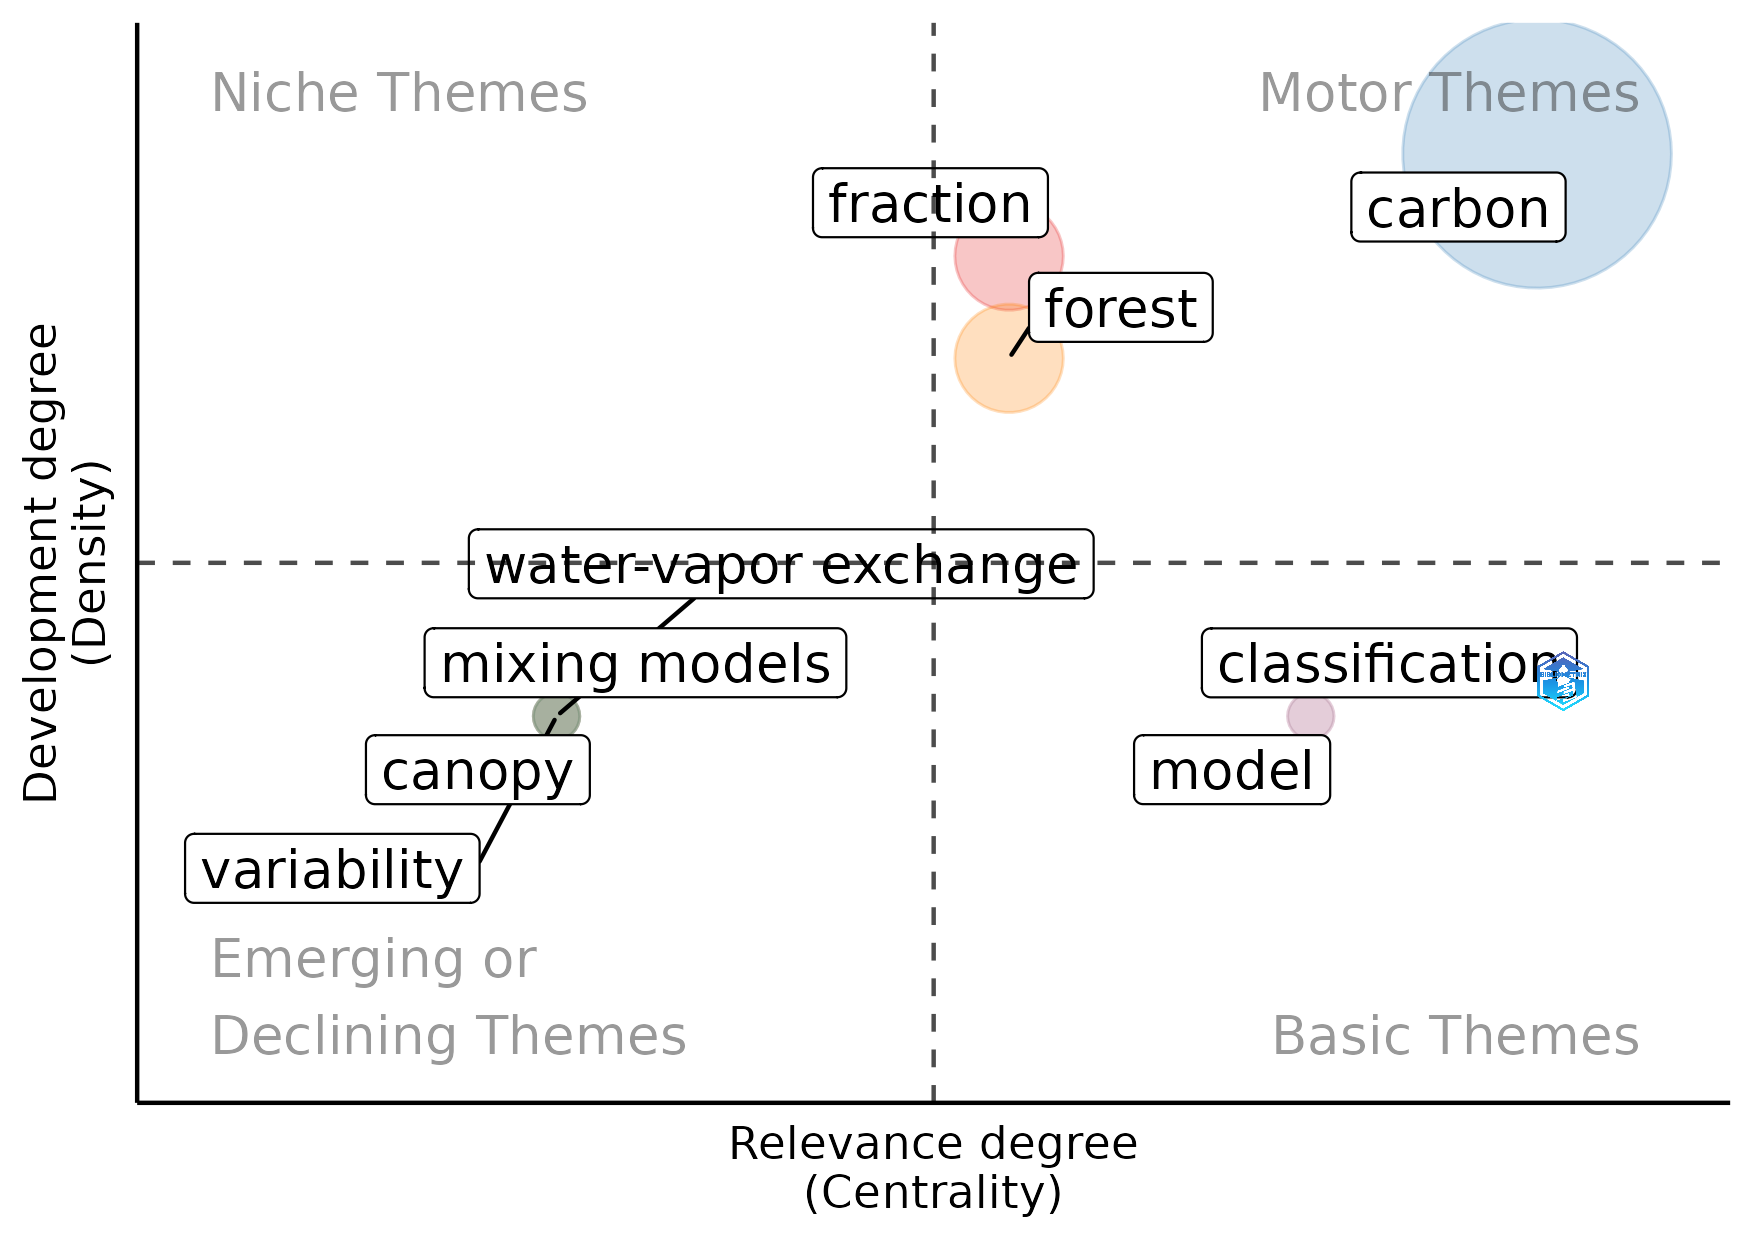
\includegraphics[width=0.7\textwidth]{figures/thematic_evolution_1.png}
    \end{figure}
\end{frame}

\begin{frame}
	\frametitle{Thematic evolution - 2008:2012}
    \begin{figure}
        \centering
        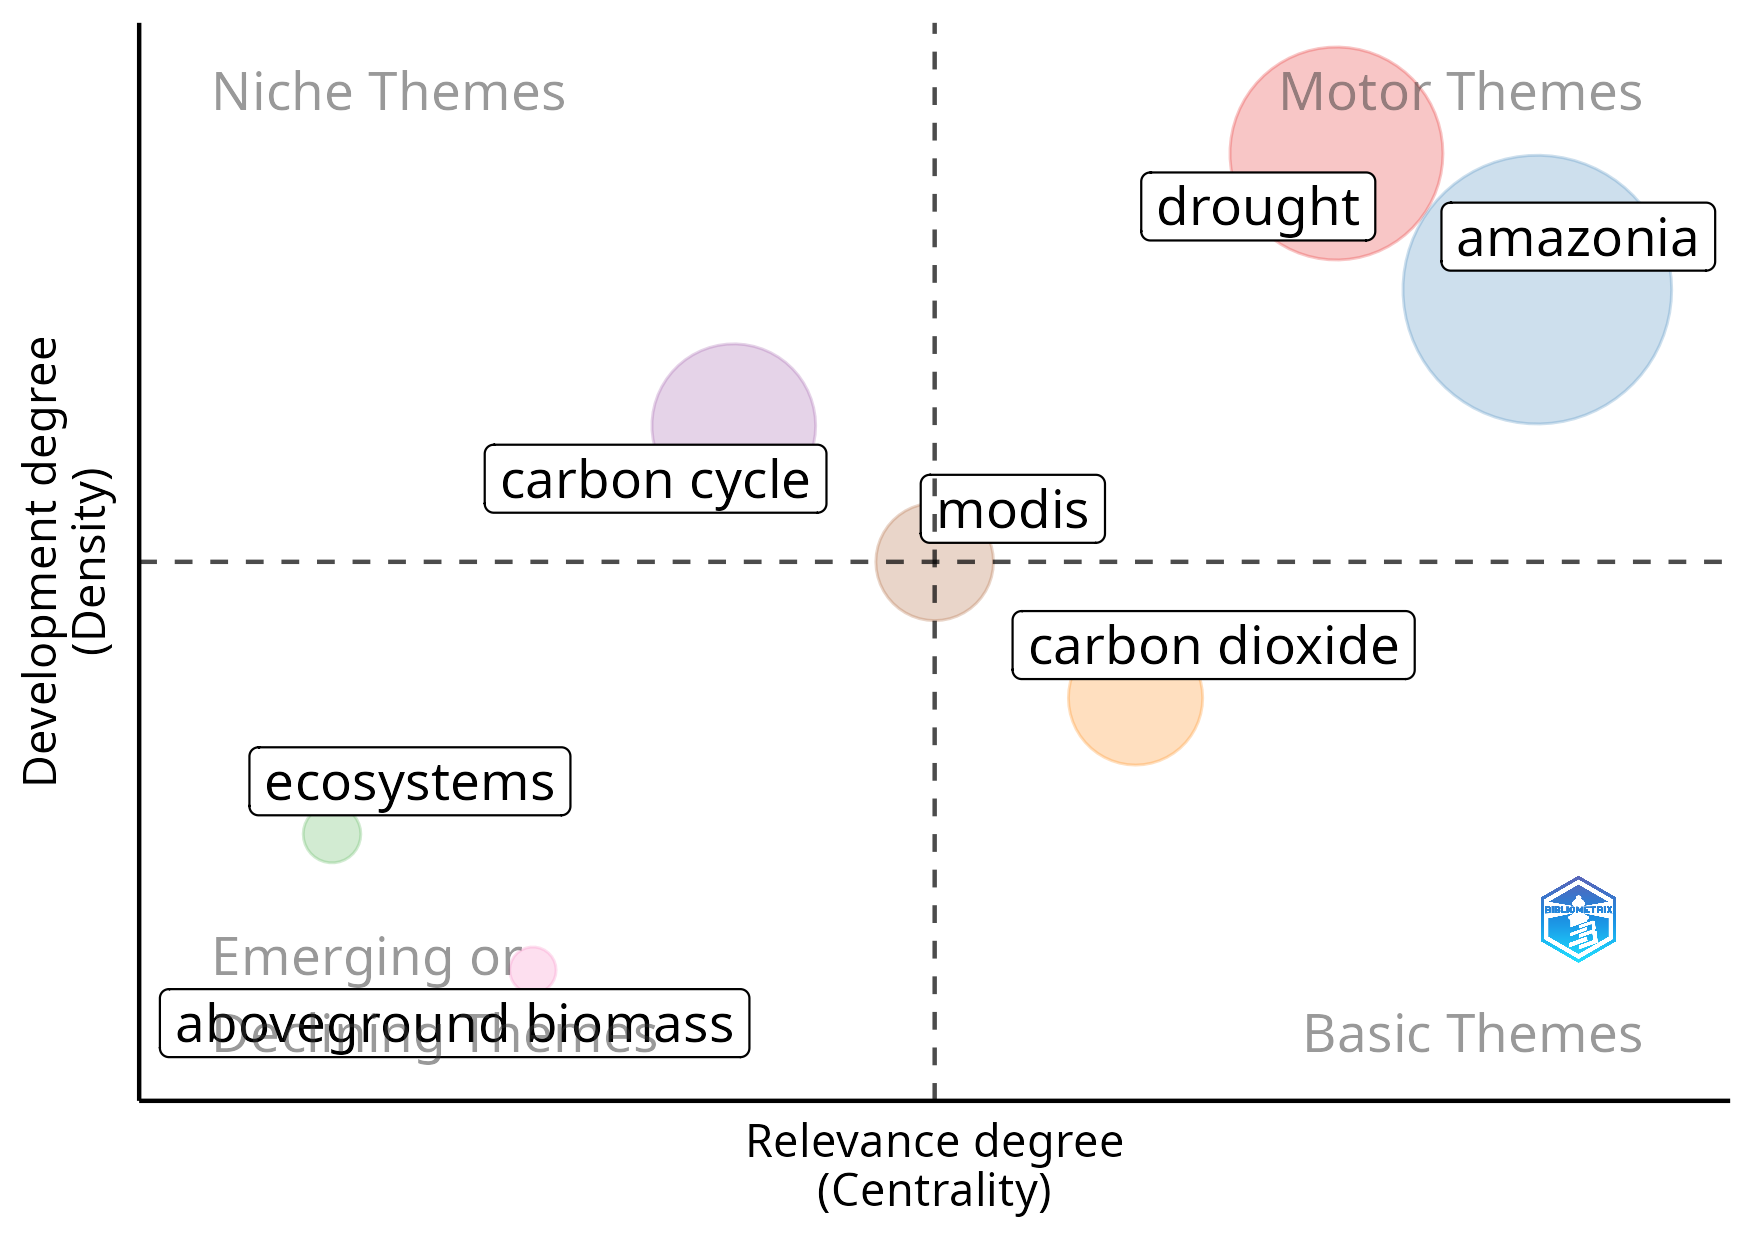
\includegraphics[width=0.7\textwidth]{figures/thematic_evolution_2.png}
    \end{figure}
\end{frame}

\begin{frame}
	\frametitle{Thematic evolution - 2013:2017}
    \begin{figure}
        \centering
        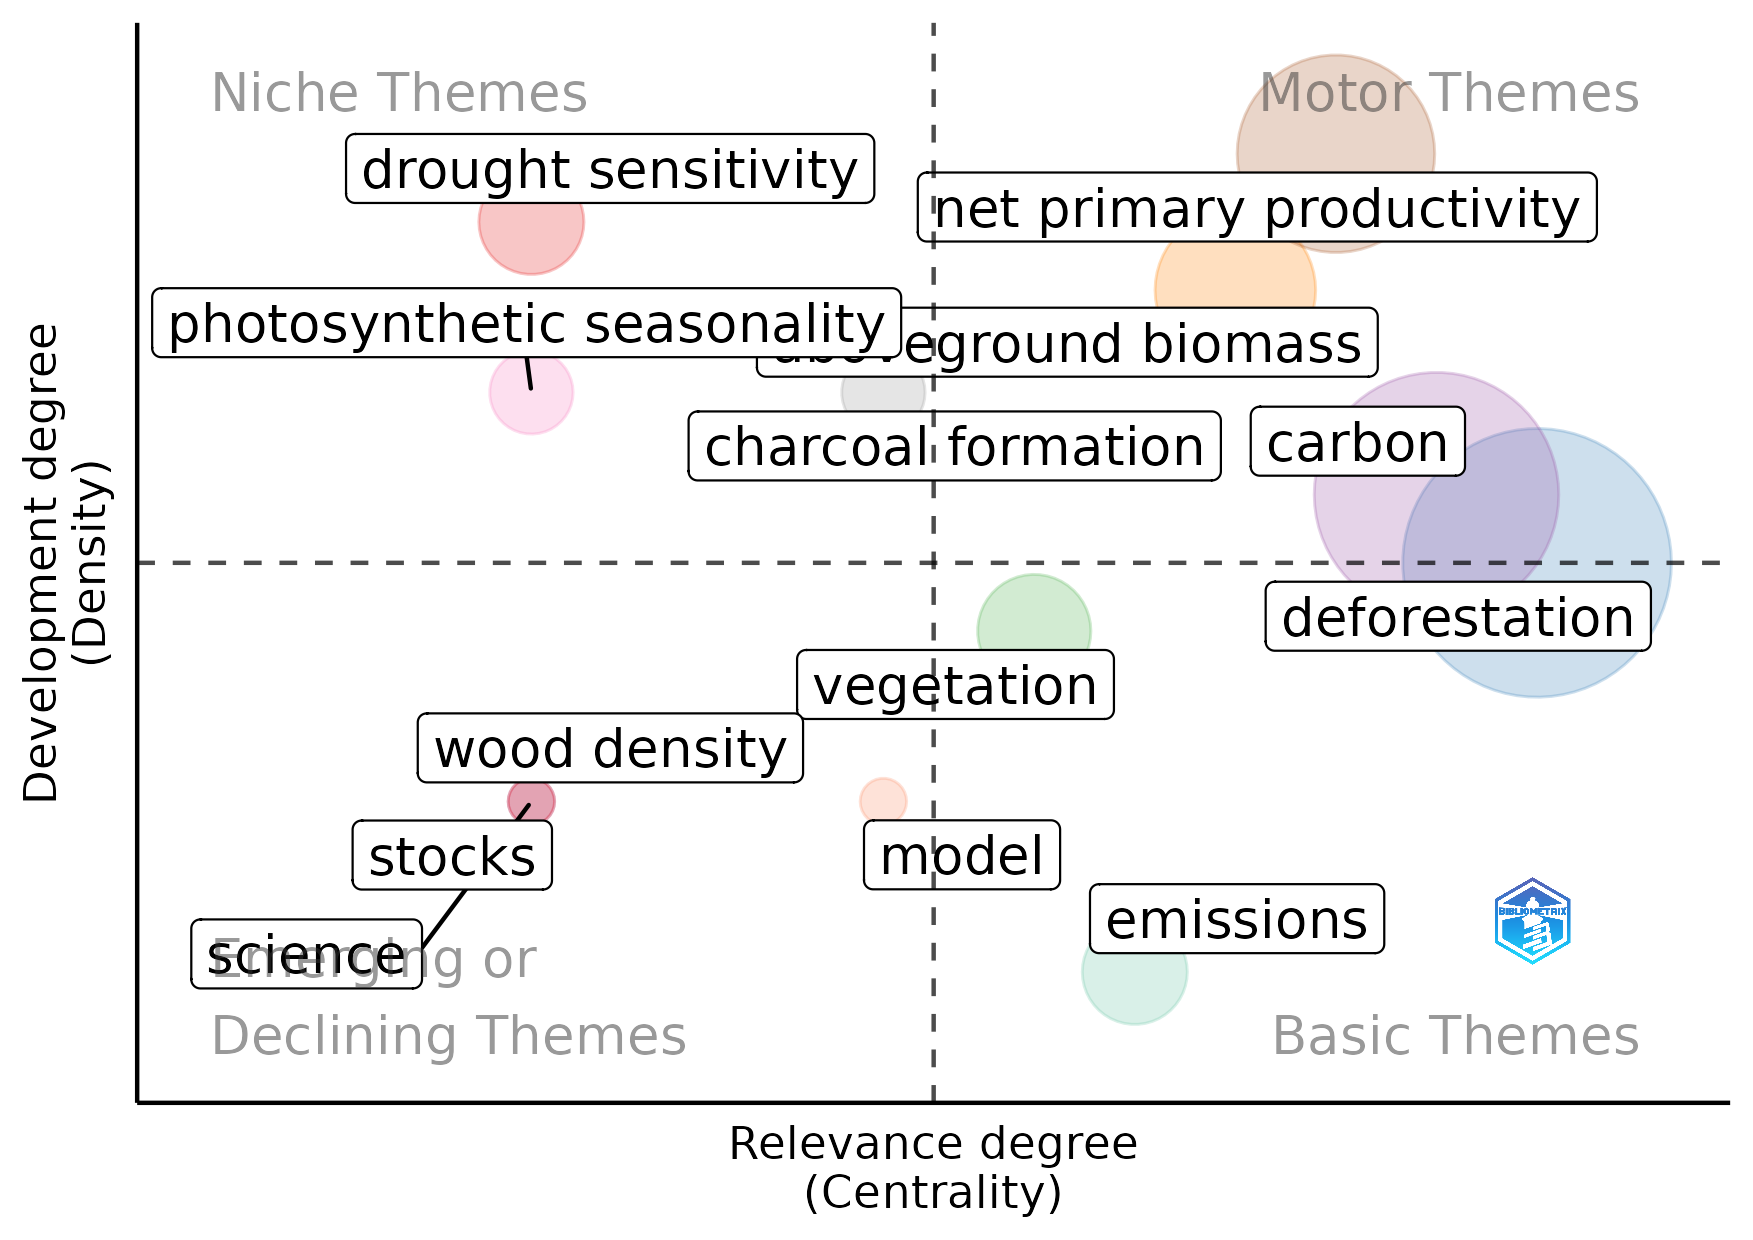
\includegraphics[width=0.7\textwidth]{figures/thematic_evolution_3.png}
    \end{figure}
\end{frame}

\begin{frame}
	\frametitle{Thematic evolution - 2018:2022}
    \begin{figure}
        \centering
        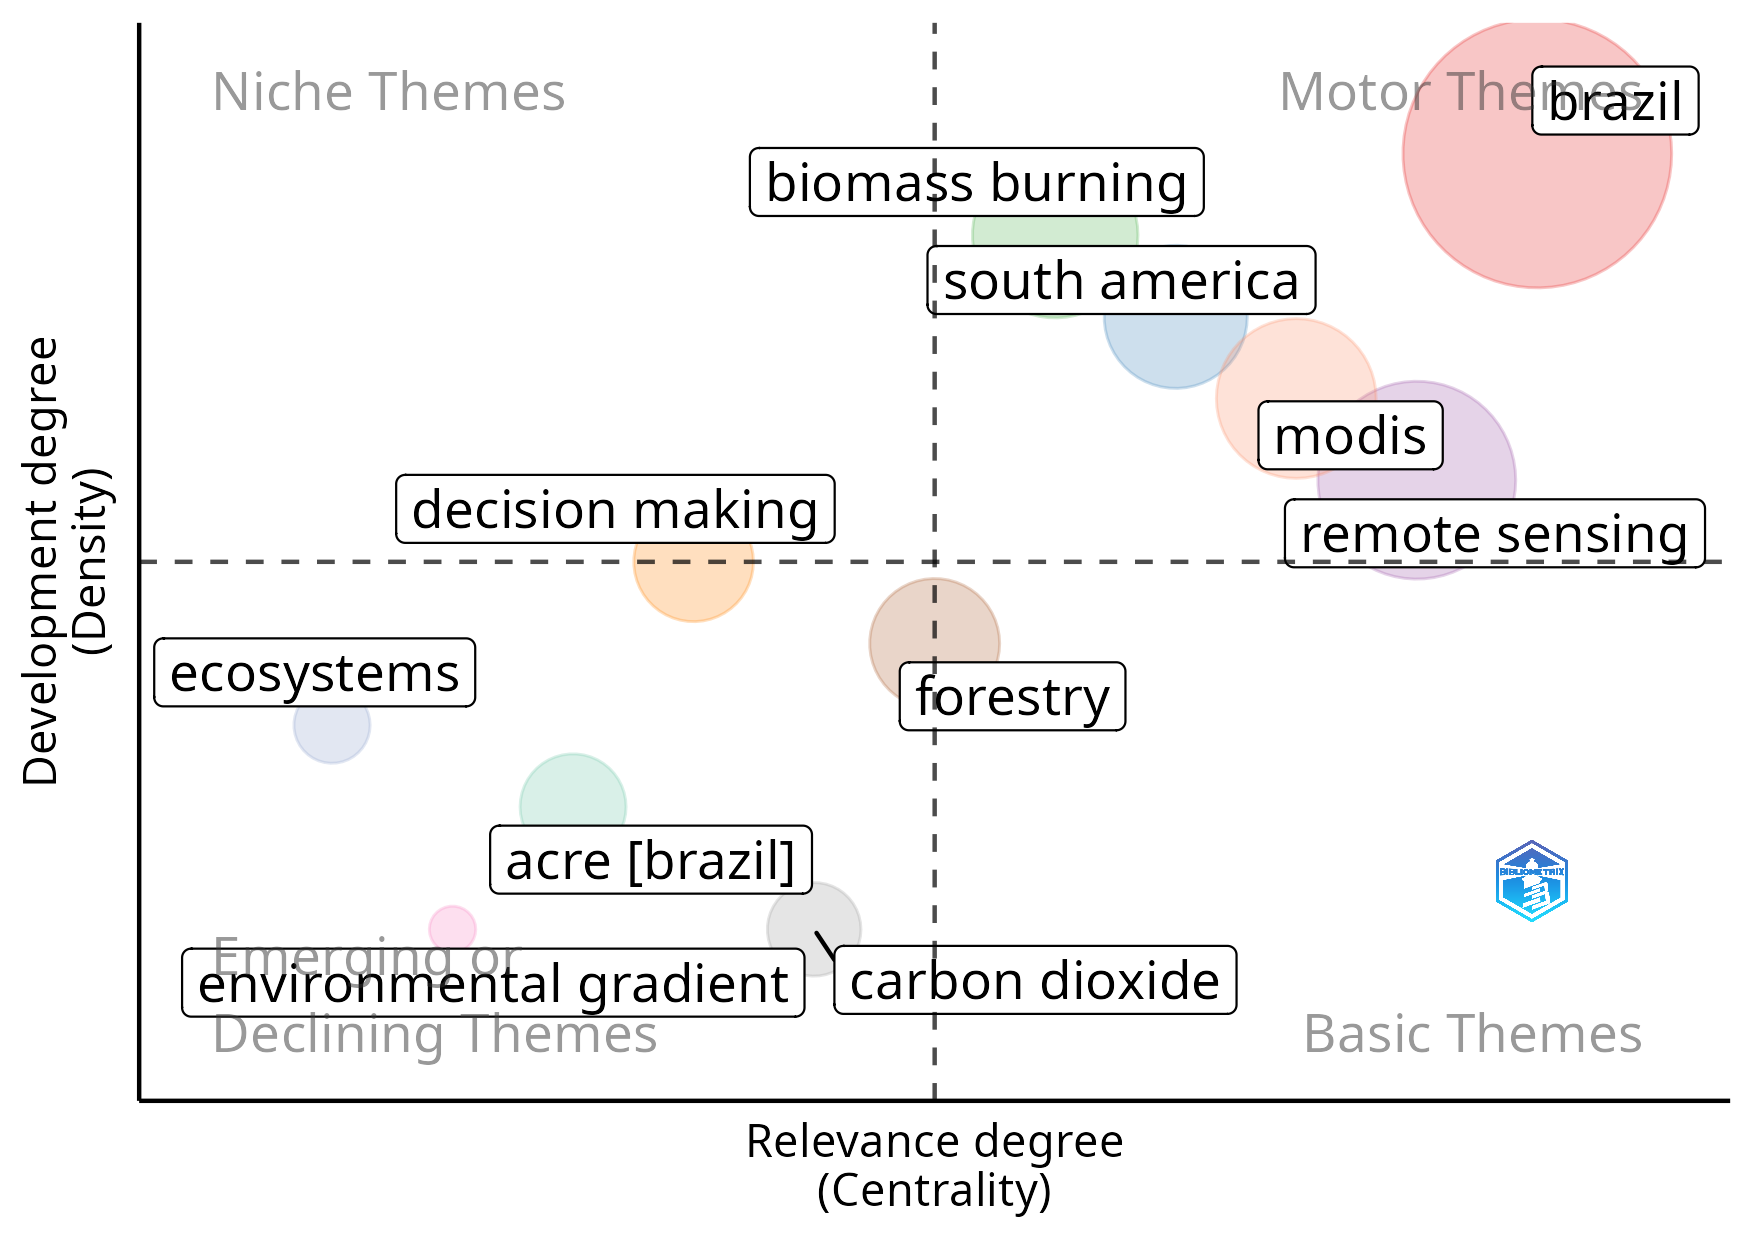
\includegraphics[width=0.7\textwidth]{figures/thematic_evolution_4.png}
    \end{figure}
\end{frame}


\subsection{Factorial analysis}


\begin{frame}
	\frametitle{Factorial Map - Most contributing documents}
	\begin{itemize}
		\item Identify the link between topic and documents.
		\item Plot the document associated to the highest absolute contribution.
		\item Absolute contributions measure the weight of each document in
		      the information summarized by the two axes.
		\item The colors represent the clusters.
	\end{itemize}
\end{frame}

\begin{frame}
	\frametitle{Factorial Map - Most contributing documents}
	\begin{itemize}
		\item Identify the link between topic and most cited documents.
		\item Plot documents associated to the highest global citations.
		\item The colors represent the clusters.
	\end{itemize}
\end{frame}

\begin{frame}
	\frametitle{Factorial Map - Most contributing documents}
	\begin{figure}
		\centering
		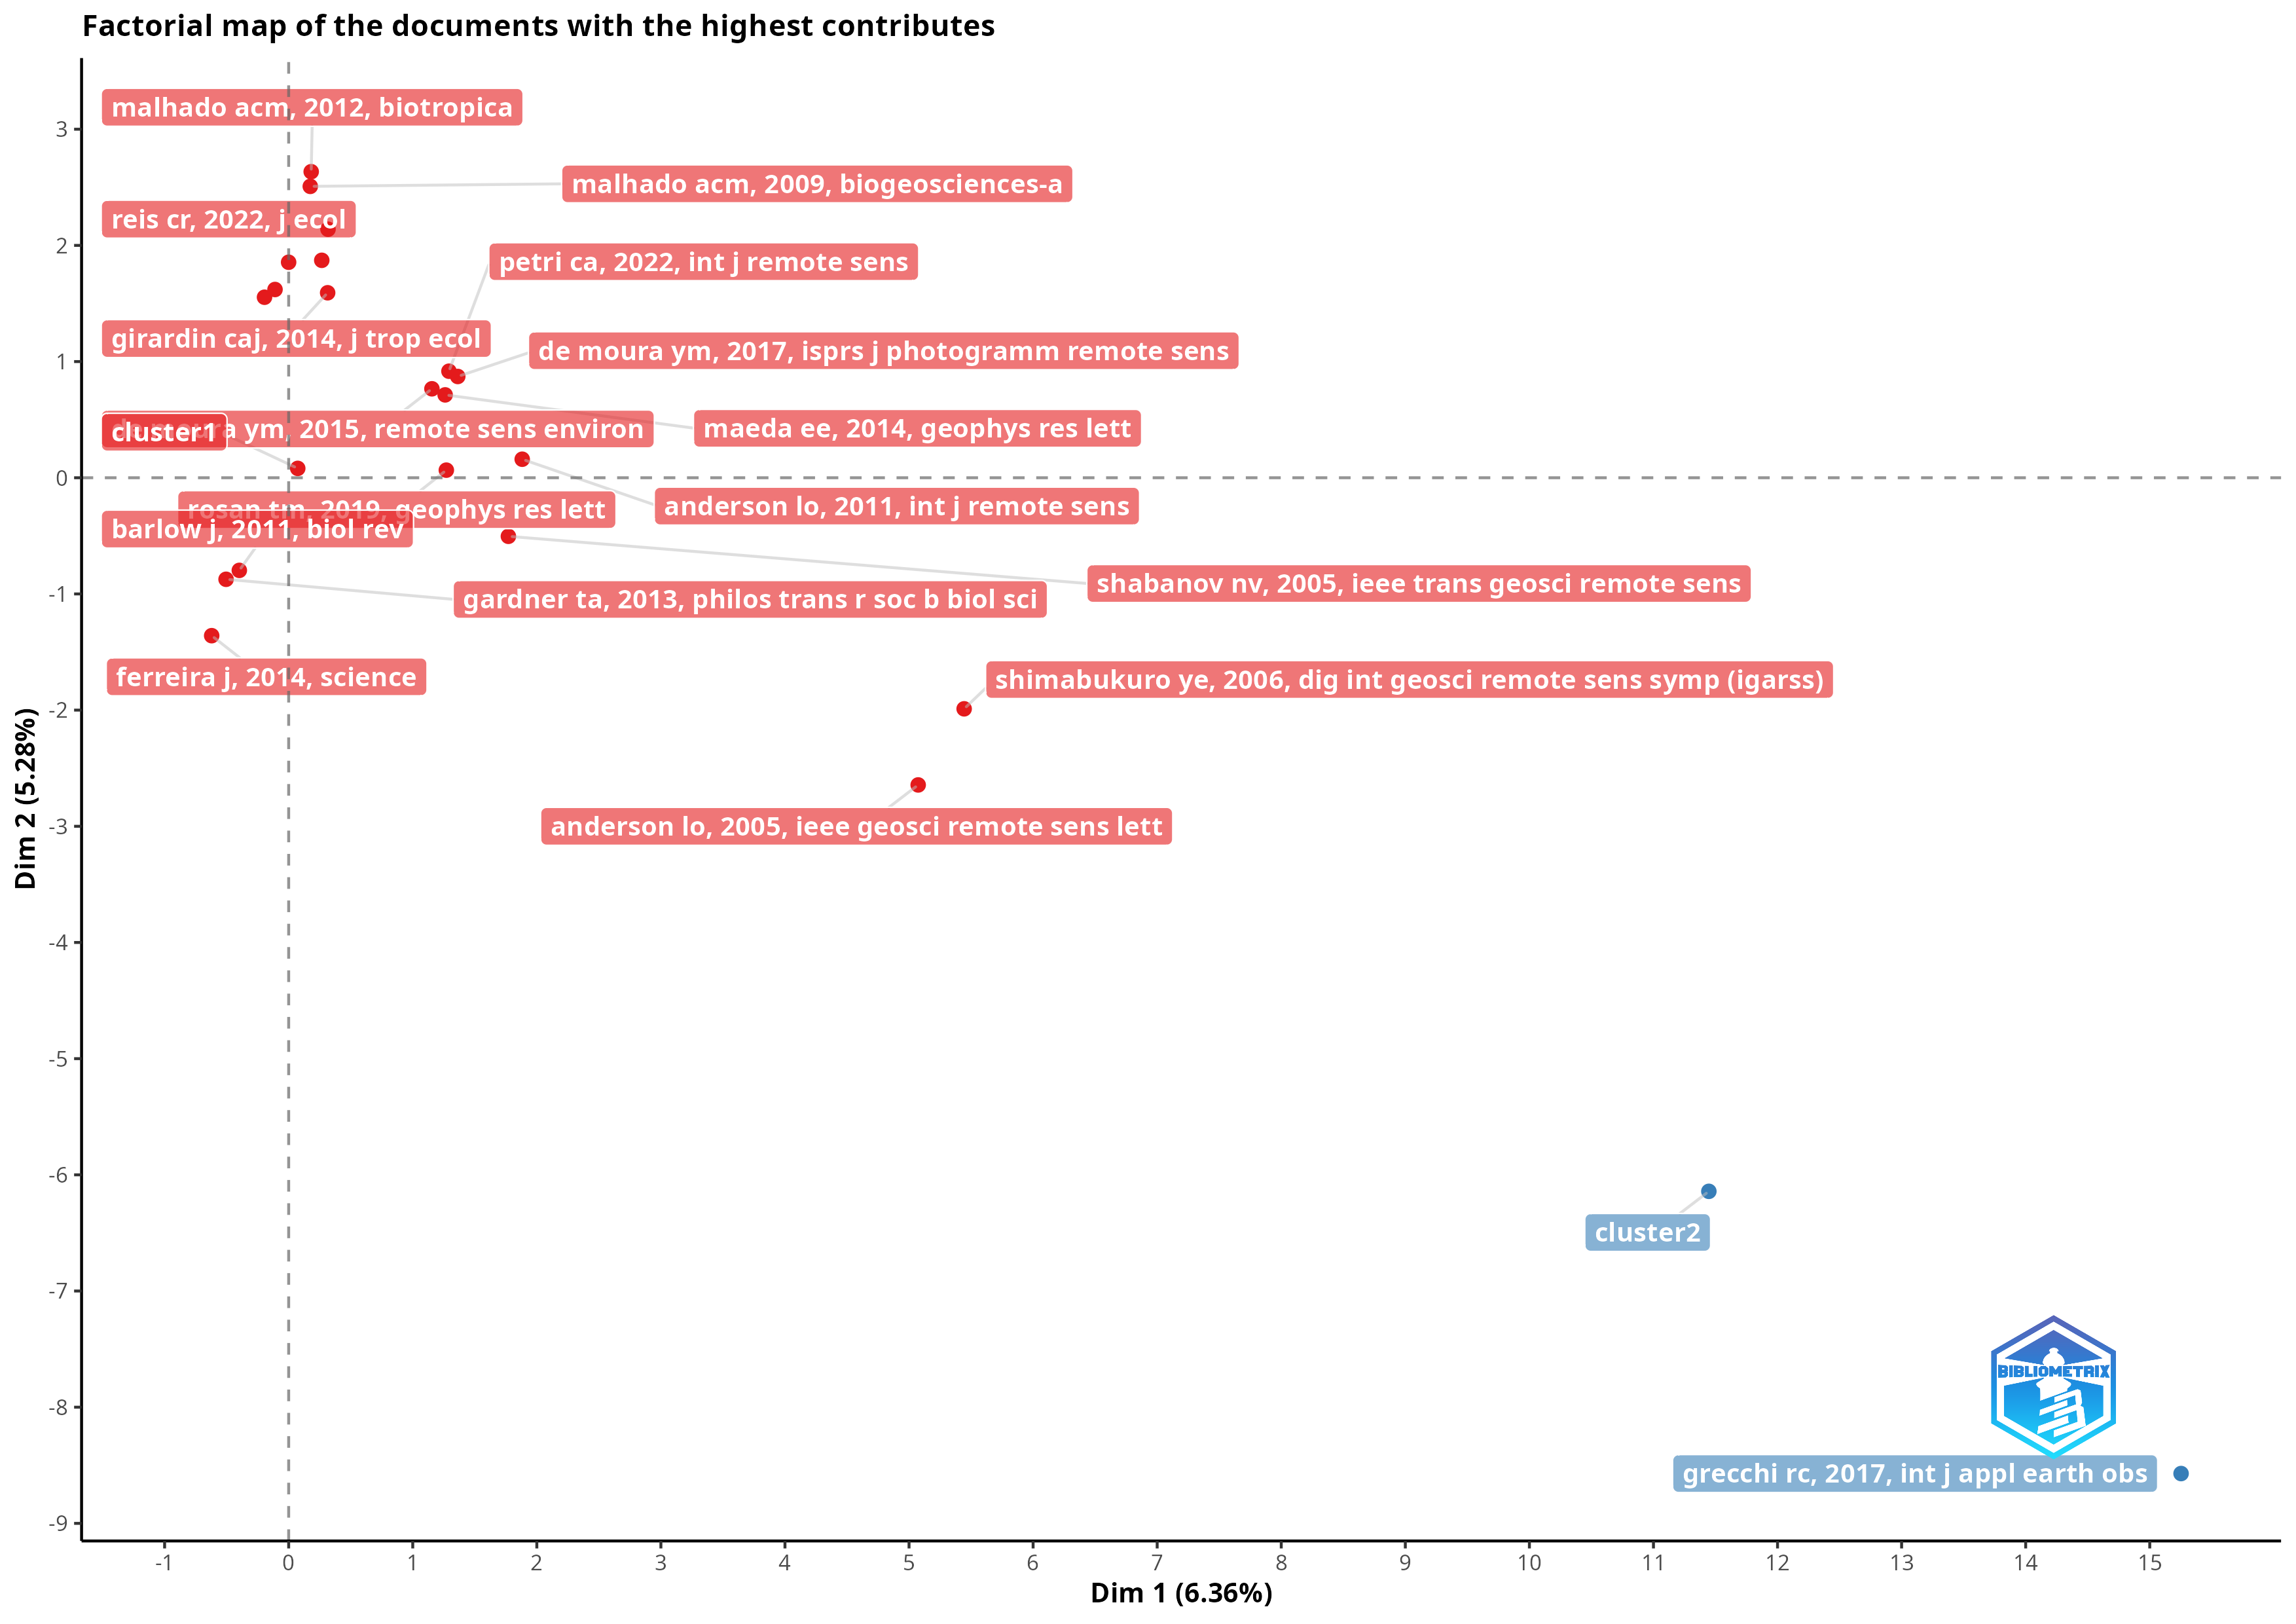
\includegraphics[width=0.7\textwidth]{figures/con_stru_map_contrib.png}
	\end{figure}
\end{frame}

\begin{frame}
	\frametitle{Factorial Map - Most cited documents}
	\begin{figure}
		\centering
		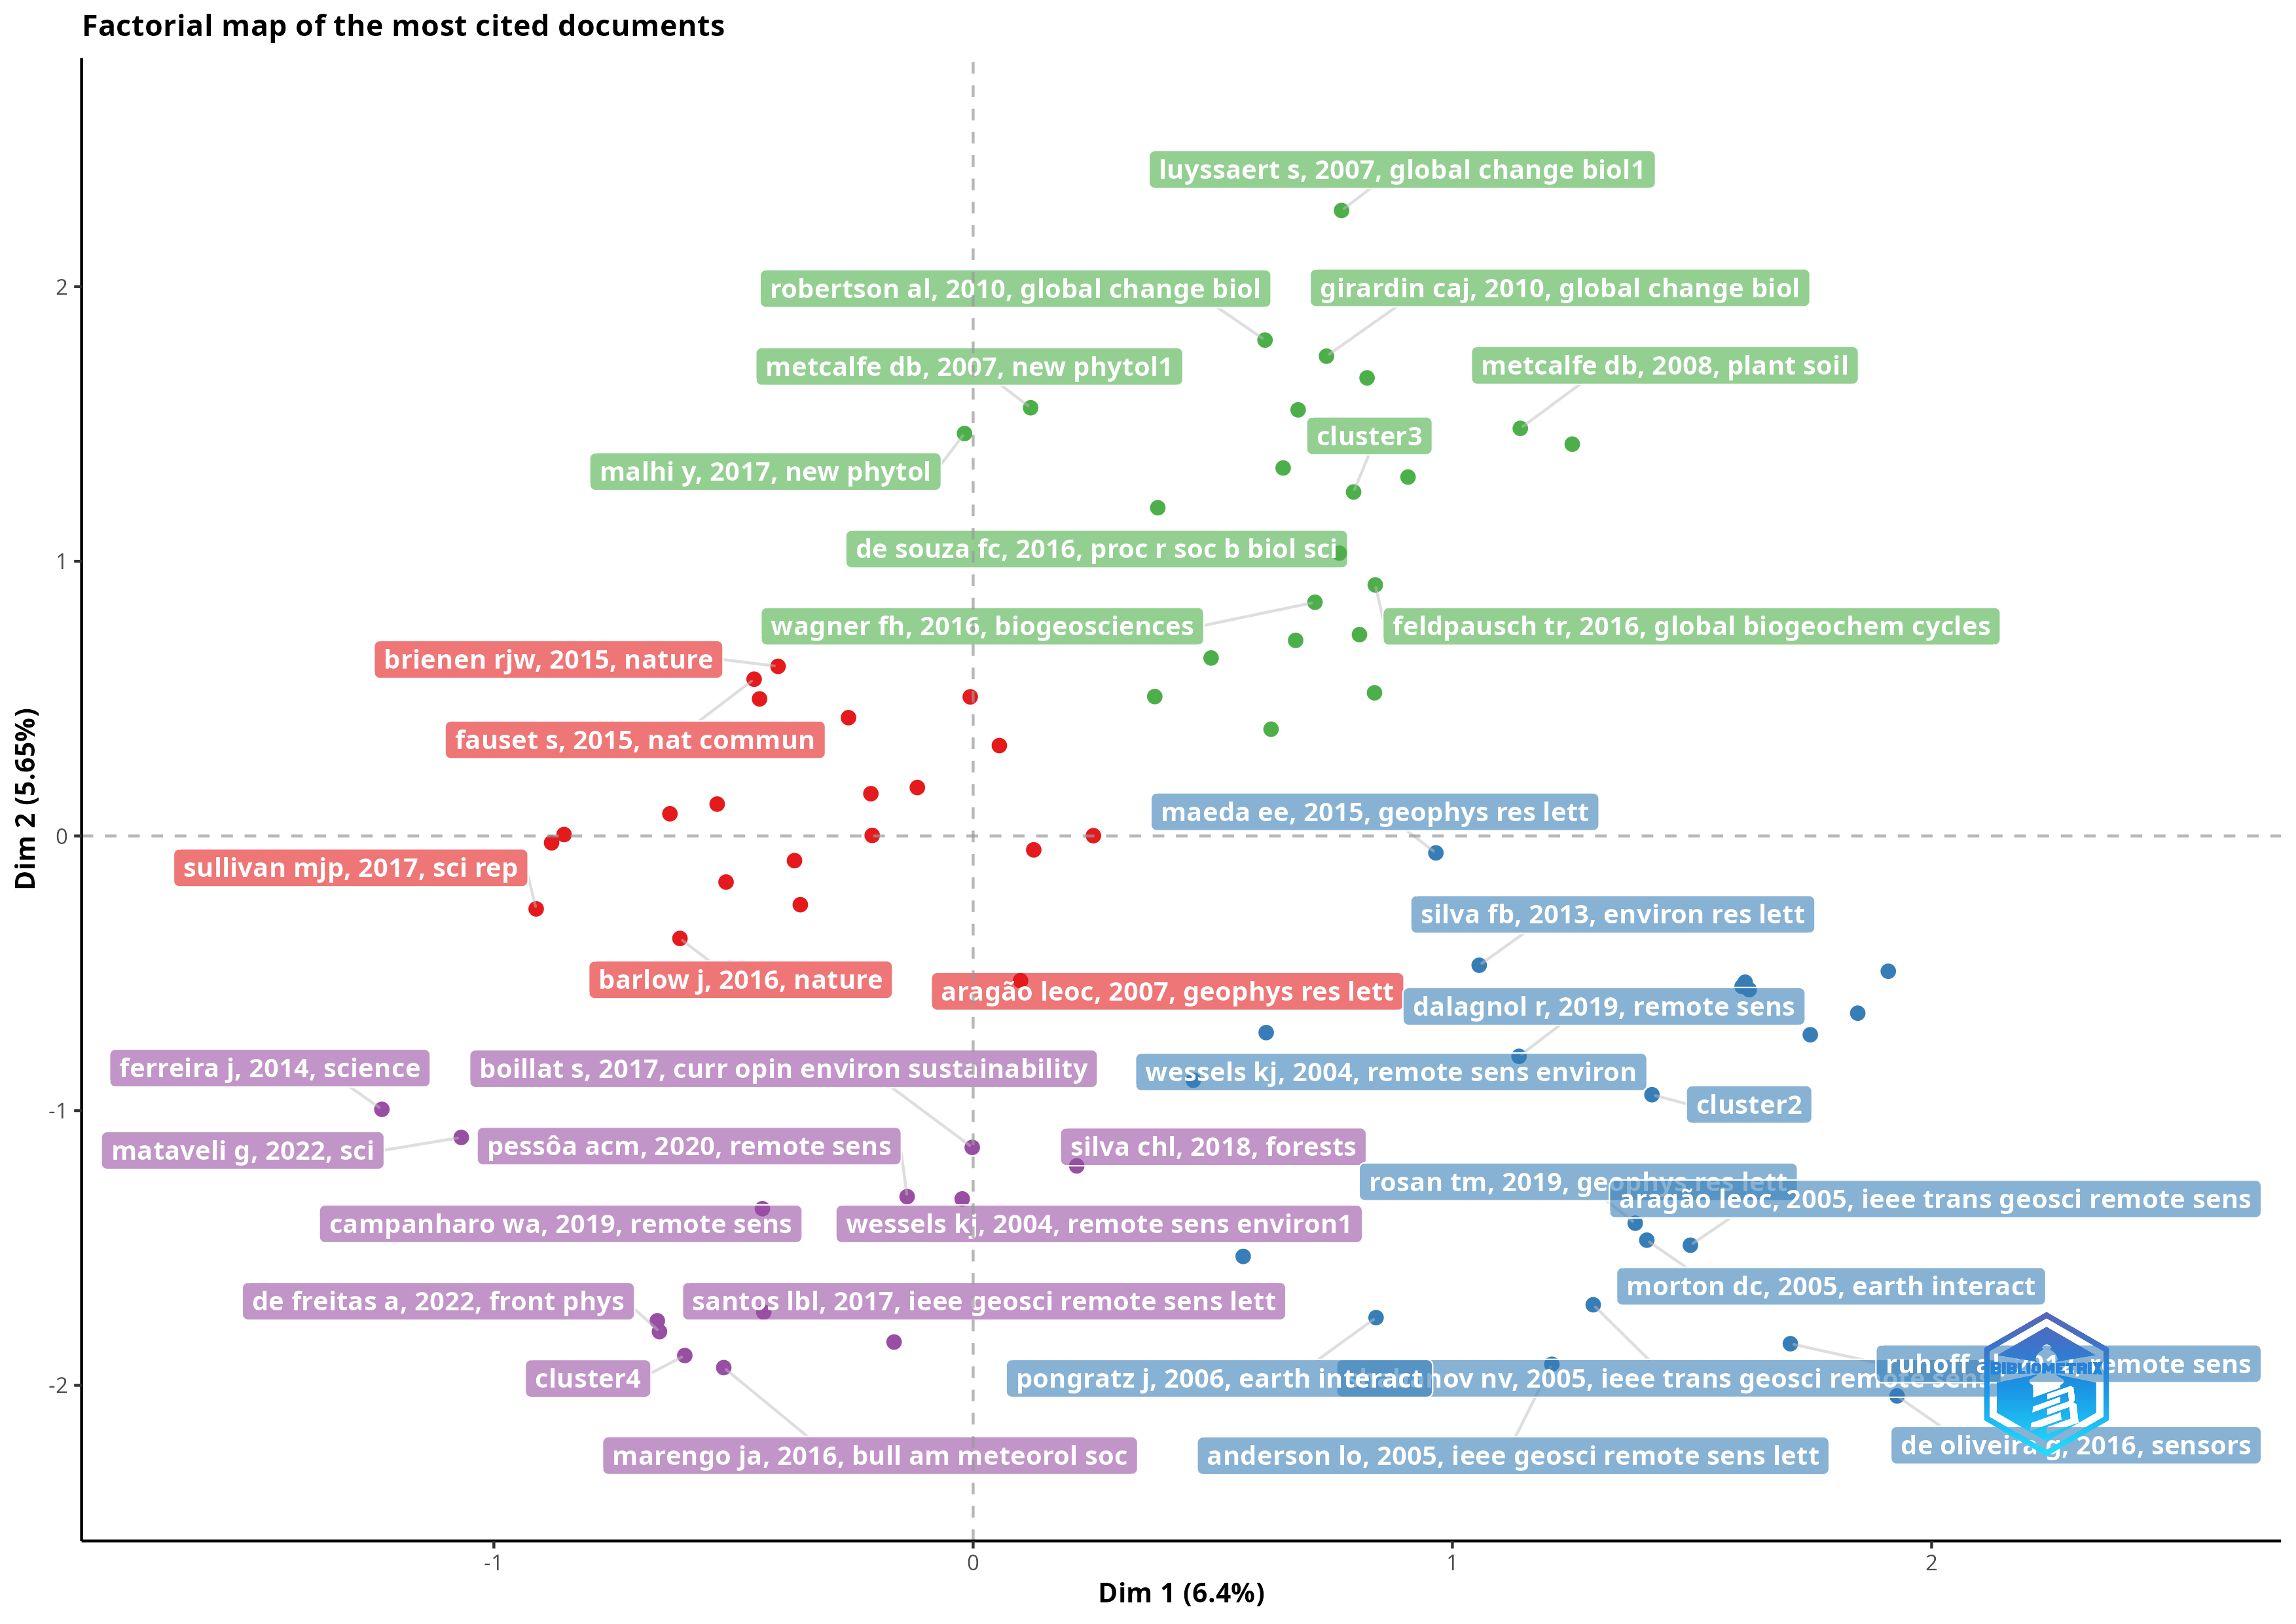
\includegraphics[width=0.7\textwidth]{figures/con_stru_map_cited.png}
	\end{figure}
\end{frame}


\subsection{Map of words}


\begin{frame}
	\frametitle{Map of words}
	\begin{itemize}
		\item Clusters are identified by hierarchical clustering.
		\item Each color corresponds to a topic.
	\end{itemize}
\end{frame}

\begin{frame}
	\frametitle{Map of words}
	\begin{figure}
		\centering
		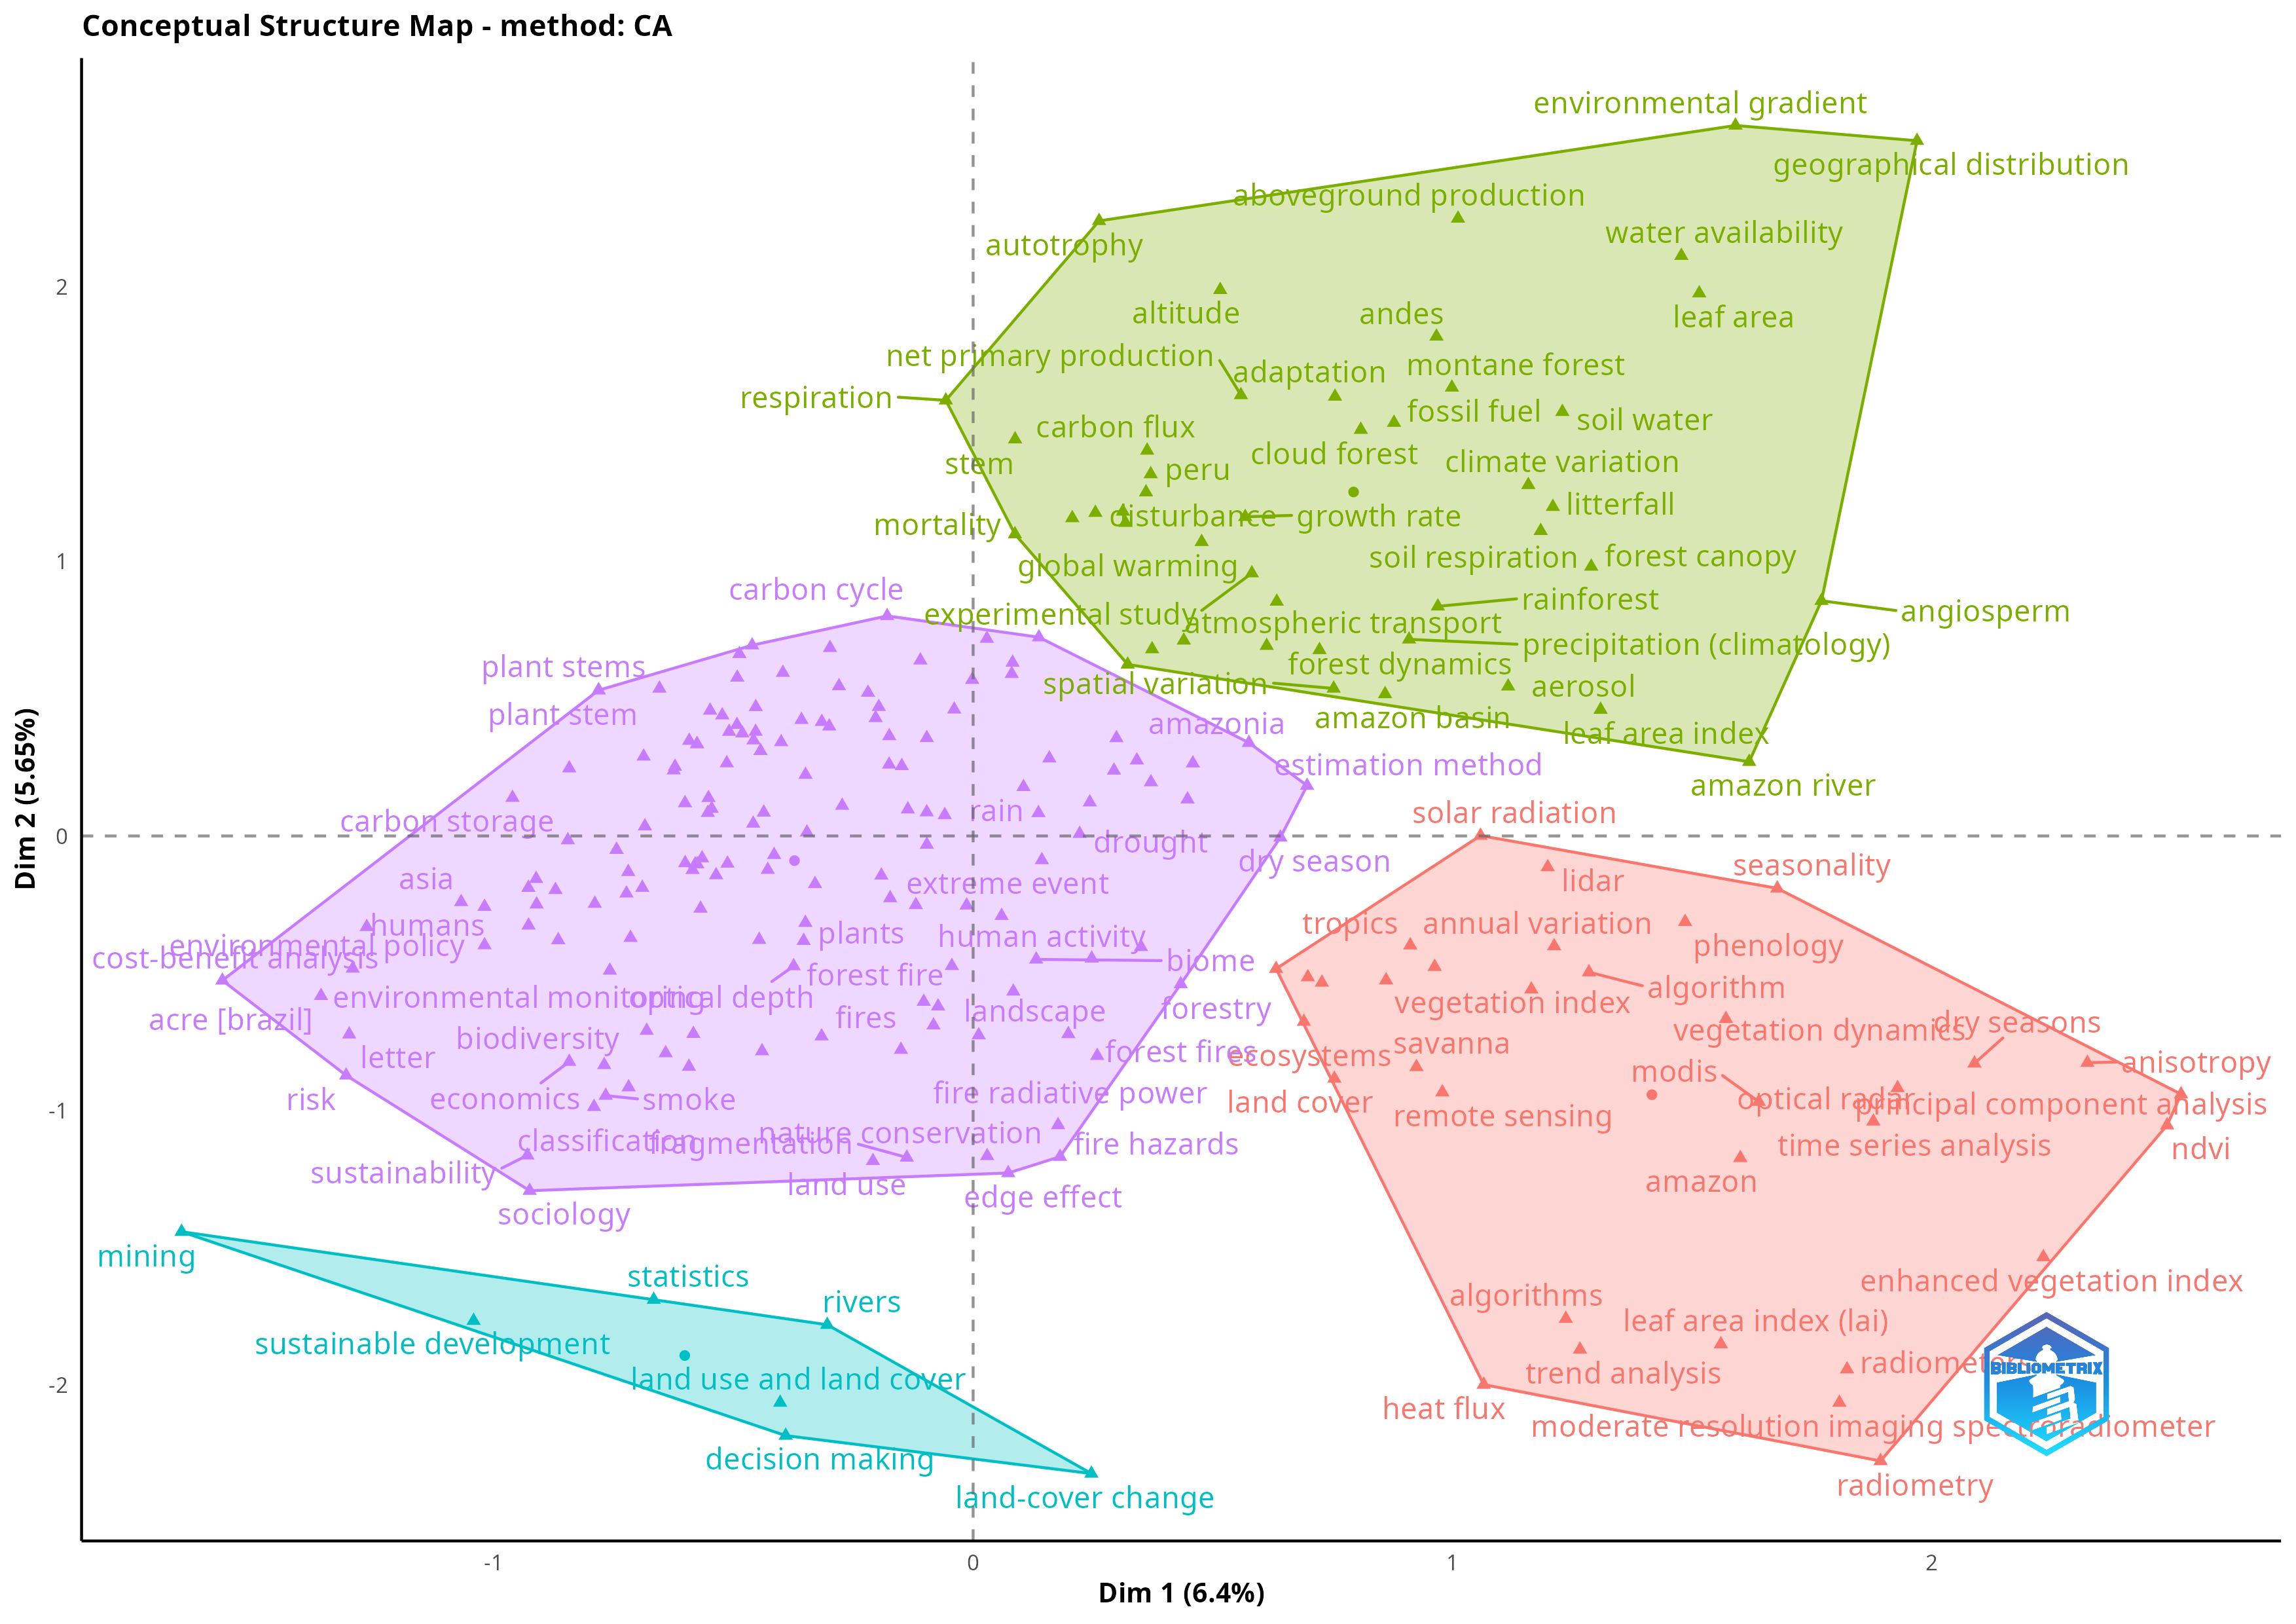
\includegraphics[width=0.7\textwidth]{figures/con_stru_map.png}
	\end{figure}
\end{frame}


\subsection{Intellectual structure}


\subsubsection{Network analysis}

\begin{frame}
	\frametitle{Network analysis}
	\begin{itemize}
		\item A network is a representation of the co-occurrence matrix.
		\item Diagonal elements are the occurrences of each item in the collection.
		\item Non-diagonal elements are the co-occurrence of two item in a
		      collection.
	\end{itemize}
\end{frame}

\begin{frame}
	\frametitle{Network - Co-occurrences Authors-Keywords}
	\begin{figure}
		\centering
		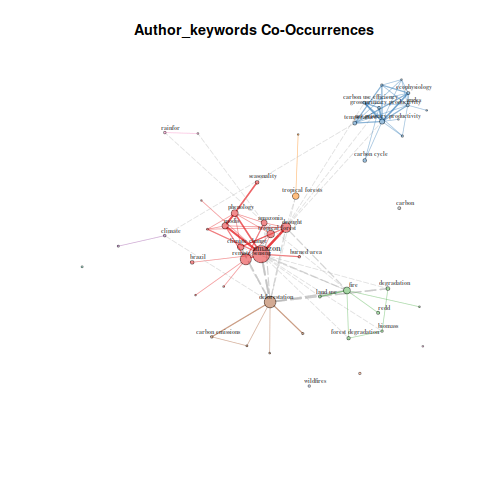
\includegraphics[width=0.5\textwidth]
		{figures/bnet_author_keywords_co-occurrences.png}
	\end{figure}
\end{frame}

\begin{frame}
	\frametitle{Network - Authors collaboration}
	\begin{figure}
		\centering
		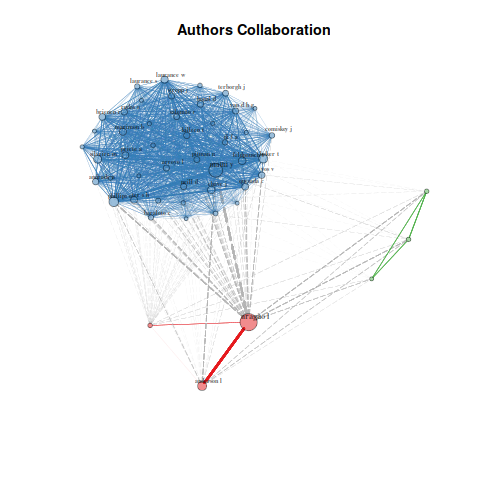
\includegraphics[width=0.5\textwidth]
		{figures/bnet_authors_collaboration.png}
	\end{figure}
\end{frame}

\begin{frame}
	\frametitle{Network - Authors co-occurrences}
	\begin{figure}
		\centering
		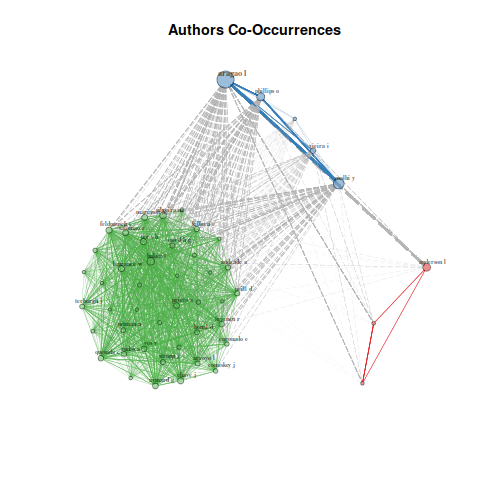
\includegraphics[width=0.5\textwidth]
		{figures/bnet_authors_co-occurrences.png}
	\end{figure}
\end{frame}

\begin{frame}
	\frametitle{Network - Authors coupling}
	\begin{figure}
		\centering
		
\includegraphics[width=0.5\textwidth]
		{figures/bnet_authors_coupling.png}
	\end{figure}
\end{frame}

\begin{frame}
	\frametitle{Network - Keyword co-occurrences}
	\begin{figure}
		\centering
		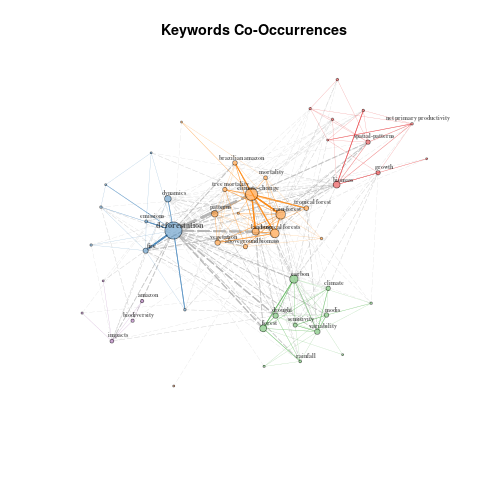
\includegraphics[width=0.5\textwidth]
		{figures/bnet_keywords_co-occurrences.png}
	\end{figure}
\end{frame}

\begin{frame}
	\frametitle{Network - References co-citation}
	\begin{figure}
		\centering
		
\includegraphics[width=0.5\textwidth]
		{figures/bnet_references_co-citation.png}
	\end{figure}
\end{frame}

\begin{frame}
	\frametitle{Network - Sources coupling}
	\begin{figure}
		\centering
		\includegraphics[width=0.5\textwidth]
		{figures/bnet_sources_coupling.png}
	\end{figure}
\end{frame}

\begin{frame}
	\frametitle{Network - Universities collaboration}
	\begin{figure}
		\centering
		\includegraphics[width=0.5\textwidth]
		{figures/bnet_universities_collaboration.png}
	\end{figure}
\end{frame}


\subsection{Social structure}


% Coupling network analysis plotted on a bi-dimensional map.

\begin{frame}
    \frametitle{Coupling network analysis (authors)}
    \begin{figure}
        \centering
        \includegraphics[width=0.7\textwidth]
        {figures/couplingmap_w_authors.png}
    \end{figure}
\end{frame}

\begin{frame}
    \frametitle{Coupling network analysis (documents)}
    \begin{figure}
        \centering
        \includegraphics[width=0.7\textwidth]
        {figures/couplingmap_w_documents.png}
    \end{figure}
\end{frame}

\begin{frame}
    \frametitle{Coupling network analysis (sources)}
    \begin{figure}
        \centering
        \includegraphics[width=0.7\textwidth]
        {figures/couplingmap_w_sources.png}
    \end{figure}
\end{frame}



\section{Summary}


\begin{frame}
	\frametitle{Take home message}
	\begin{itemize}
		\item It's healthy for TreesLab to look at itself once in a while. 
        \item An introspection excercise reveals trends and patterns along 20 
            years of research, spotting ways to move forward.
        \item The tools and services presented here, can be chained for 
            regular reporting and monitoring. 
        \item Besides, these tools allow exploring new or converging 
            knowledge areas, easing the TreesLab path into potential 
            opportunities in interdisciplinar research.
	\end{itemize}
\end{frame}

\begin{frame}[allowframebreaks]
	\frametitle{References}
	\printbibliography
\end{frame}

\end{document}

